\documentclass[14pt,ignorenonframetext,]{bredelebeamer}
\setbeamertemplate{caption}[numbered]
\setbeamertemplate{caption label separator}{: }
\setbeamercolor{caption name}{fg=normal text.fg}
\beamertemplatenavigationsymbolsempty
\usepackage{lmodern}
\usepackage{amssymb,amsmath}
\usepackage{ifxetex,ifluatex}
\usepackage{fixltx2e} % provides \textsubscript
\ifnum 0\ifxetex 1\fi\ifluatex 1\fi=0 % if pdftex
  \usepackage[T1]{fontenc}
  \usepackage[utf8]{inputenc}
\else % if luatex or xelatex
  \ifxetex
    \usepackage{mathspec}
  \else
    \usepackage{fontspec}
  \fi
  \defaultfontfeatures{Ligatures=TeX,Scale=MatchLowercase}
\fi
% use upquote if available, for straight quotes in verbatim environments
\IfFileExists{upquote.sty}{\usepackage{upquote}}{}
% use microtype if available
\IfFileExists{microtype.sty}{%
\usepackage{microtype}
\UseMicrotypeSet[protrusion]{basicmath} % disable protrusion for tt fonts
}{}
\newif\ifbibliography
\hypersetup{
            pdftitle={Journal Club Bioinfo},
            pdfauthor={ROCHER Vincent},
            pdfborder={0 0 0},
            breaklinks=true}
\urlstyle{same}  % don't use monospace font for urls
\usepackage{color}
\usepackage{fancyvrb}
\newcommand{\VerbBar}{|}
\newcommand{\VERB}{\Verb[commandchars=\\\{\}]}
\DefineVerbatimEnvironment{Highlighting}{Verbatim}{commandchars=\\\{\}}
% Add ',fontsize=\small' for more characters per line
\usepackage{framed}
\definecolor{shadecolor}{RGB}{48,48,48}
\newenvironment{Shaded}{\begin{snugshade}}{\end{snugshade}}
\newcommand{\KeywordTok}[1]{\textcolor[rgb]{0.94,0.87,0.69}{#1}}
\newcommand{\DataTypeTok}[1]{\textcolor[rgb]{0.87,0.87,0.75}{#1}}
\newcommand{\DecValTok}[1]{\textcolor[rgb]{0.86,0.86,0.80}{#1}}
\newcommand{\BaseNTok}[1]{\textcolor[rgb]{0.86,0.64,0.64}{#1}}
\newcommand{\FloatTok}[1]{\textcolor[rgb]{0.75,0.75,0.82}{#1}}
\newcommand{\ConstantTok}[1]{\textcolor[rgb]{0.86,0.64,0.64}{\textbf{#1}}}
\newcommand{\CharTok}[1]{\textcolor[rgb]{0.86,0.64,0.64}{#1}}
\newcommand{\SpecialCharTok}[1]{\textcolor[rgb]{0.86,0.64,0.64}{#1}}
\newcommand{\StringTok}[1]{\textcolor[rgb]{0.80,0.58,0.58}{#1}}
\newcommand{\VerbatimStringTok}[1]{\textcolor[rgb]{0.80,0.58,0.58}{#1}}
\newcommand{\SpecialStringTok}[1]{\textcolor[rgb]{0.80,0.58,0.58}{#1}}
\newcommand{\ImportTok}[1]{\textcolor[rgb]{0.80,0.80,0.80}{#1}}
\newcommand{\CommentTok}[1]{\textcolor[rgb]{0.50,0.62,0.50}{#1}}
\newcommand{\DocumentationTok}[1]{\textcolor[rgb]{0.50,0.62,0.50}{#1}}
\newcommand{\AnnotationTok}[1]{\textcolor[rgb]{0.50,0.62,0.50}{\textbf{#1}}}
\newcommand{\CommentVarTok}[1]{\textcolor[rgb]{0.50,0.62,0.50}{\textbf{#1}}}
\newcommand{\OtherTok}[1]{\textcolor[rgb]{0.94,0.94,0.56}{#1}}
\newcommand{\FunctionTok}[1]{\textcolor[rgb]{0.94,0.94,0.56}{#1}}
\newcommand{\VariableTok}[1]{\textcolor[rgb]{0.80,0.80,0.80}{#1}}
\newcommand{\ControlFlowTok}[1]{\textcolor[rgb]{0.94,0.87,0.69}{#1}}
\newcommand{\OperatorTok}[1]{\textcolor[rgb]{0.94,0.94,0.82}{#1}}
\newcommand{\BuiltInTok}[1]{\textcolor[rgb]{0.80,0.80,0.80}{#1}}
\newcommand{\ExtensionTok}[1]{\textcolor[rgb]{0.80,0.80,0.80}{#1}}
\newcommand{\PreprocessorTok}[1]{\textcolor[rgb]{1.00,0.81,0.69}{\textbf{#1}}}
\newcommand{\AttributeTok}[1]{\textcolor[rgb]{0.80,0.80,0.80}{#1}}
\newcommand{\RegionMarkerTok}[1]{\textcolor[rgb]{0.80,0.80,0.80}{#1}}
\newcommand{\InformationTok}[1]{\textcolor[rgb]{0.50,0.62,0.50}{\textbf{#1}}}
\newcommand{\WarningTok}[1]{\textcolor[rgb]{0.50,0.62,0.50}{\textbf{#1}}}
\newcommand{\AlertTok}[1]{\textcolor[rgb]{1.00,0.81,0.69}{#1}}
\newcommand{\ErrorTok}[1]{\textcolor[rgb]{0.76,0.75,0.62}{#1}}
\newcommand{\NormalTok}[1]{\textcolor[rgb]{0.80,0.80,0.80}{#1}}
\usepackage{graphicx,grffile}
\makeatletter
\def\maxwidth{\ifdim\Gin@nat@width>\linewidth\linewidth\else\Gin@nat@width\fi}
\def\maxheight{\ifdim\Gin@nat@height>\textheight0.8\textheight\else\Gin@nat@height\fi}
\makeatother
% Scale images if necessary, so that they will not overflow the page
% margins by default, and it is still possible to overwrite the defaults
% using explicit options in \includegraphics[width, height, ...]{}
\setkeys{Gin}{width=\maxwidth,height=\maxheight,keepaspectratio}

% Prevent slide breaks in the middle of a paragraph:
\widowpenalties 1 10000
\raggedbottom

\AtBeginPart{
  \let\insertpartnumber\relax
  \let\partname\relax
  \frame{\partpage}
}
\AtBeginSection{
  \ifbibliography
  \else
    \let\insertsectionnumber\relax
    \let\sectionname\relax
    \frame{\sectionpage}
  \fi
}
\AtBeginSubsection{
  \let\insertsubsectionnumber\relax
  \let\subsectionname\relax
  \frame{\subsectionpage}
}

\setlength{\parindent}{0pt}
\setlength{\parskip}{6pt plus 2pt minus 1pt}
\setlength{\emergencystretch}{3em}  % prevent overfull lines
\providecommand{\tightlist}{%
  \setlength{\itemsep}{0pt}\setlength{\parskip}{0pt}}
\setcounter{secnumdepth}{0}

\title{Journal Club Bioinfo}
\subtitle{\textbf{The Tidyverse}: A collection of R packages designed for data
science.}
\author{ROCHER Vincent}
\date{28 mars 2019}

\begin{document}
\frame{\titlepage}

\begin{frame}{R for data science}
\begin{columns}
    \begin{column}{0.3\textwidth}

\includegraphics{images/cover.png}
    \end{column}
    \begin{column}{0.7\textwidth}
    \begin{Large}
    \begin{itemize}
        \item \textbf{R for data science}: The best place to start learning the tidyverse by Hadley Wickham and Garrett Grolemund\footnote{available online : \url{https://r4ds.had.co.nz}.}.
        \item \textbf{ggplot2: elegant graphics for data science} by Hadley Wickham. Goes into greater depth into the ggplot2 visualisation system.
    \end{itemize}
    \end{Large}
    \end{column}
\end{columns}
\end{frame}

\begin{frame}
\tableofcontents[hideallsubsections]
\end{frame}

\section{Tidyverse \& tidy data}\label{tidyverse-tidy-data}

\begin{frame}[fragile]{Tidyverse}

\begin{columns}
    \begin{column}{0.3\textwidth}
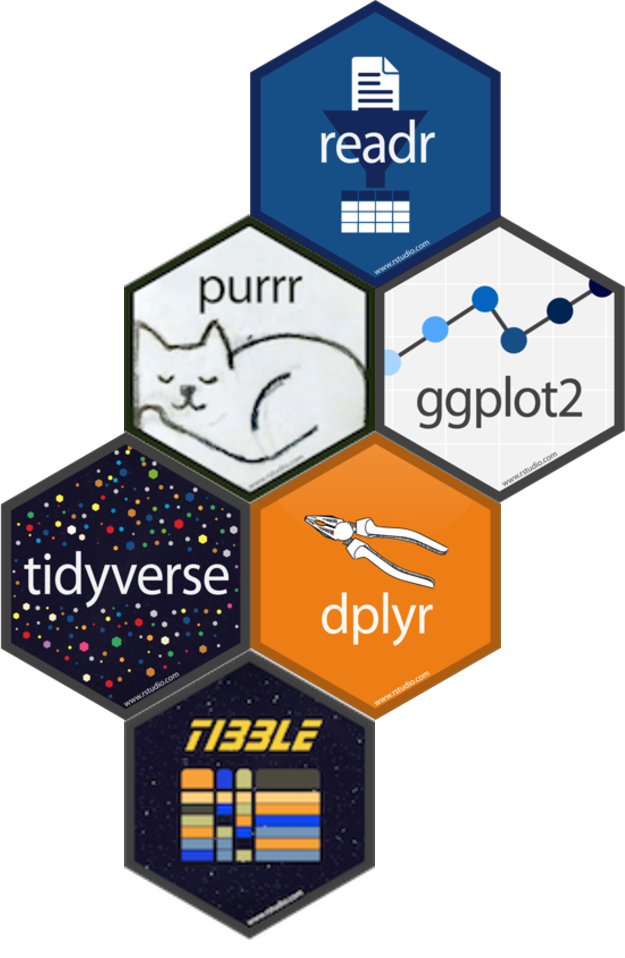
\includegraphics{images/Tidyverse.pdf}
    \end{column}
    \begin{column}{0.7\textwidth}
    \begin{Huge}
        \textbf{R packages for data science}
    \end{Huge}
    
    \begin{Large}
        The tidyverse is an opinionated collection of R packages designed for data science. All packages share an underlying design philosophy, grammar, and data structures.\\
        \url{https://www.tidyverse.org/}
    \end{Large}


    
    \end{column}
\end{columns}

\begin{Shaded}
\begin{Highlighting}[]
\KeywordTok{install.packages}\NormalTok{(}\StringTok{"tidyverse"}\NormalTok{)}
\end{Highlighting}
\end{Shaded}

\end{frame}

\begin{frame}[fragile]{Tidyverse}

\small

\begin{Shaded}
\begin{Highlighting}[]
\KeywordTok{require}\NormalTok{(tidyverse)}
\end{Highlighting}
\end{Shaded}

\begin{verbatim}
## Loading required package: tidyverse
\end{verbatim}

\begin{verbatim}
## -- Attaching packages ----------------------------------------------- tidyverse 1.2.1 --
\end{verbatim}

\begin{verbatim}
## v ggplot2 3.1.0     v purrr   0.2.5
## v tibble  2.0.1     v dplyr   0.7.8
## v tidyr   0.8.2     v stringr 1.4.0
## v readr   1.3.1     v forcats 0.3.0
\end{verbatim}

\begin{verbatim}
## -- Conflicts -------------------------------------------------- tidyverse_conflicts() --
## x dplyr::filter() masks stats::filter()
## x dplyr::lag()    masks stats::lag()
\end{verbatim}

\end{frame}

\begin{frame}{Tidy data}

\begin{Large}
\textit{\textbf{Tidying:} structuring datasets to facilitate analysis.}
\end{Large}\begin{center}
A tidy dataset :\\
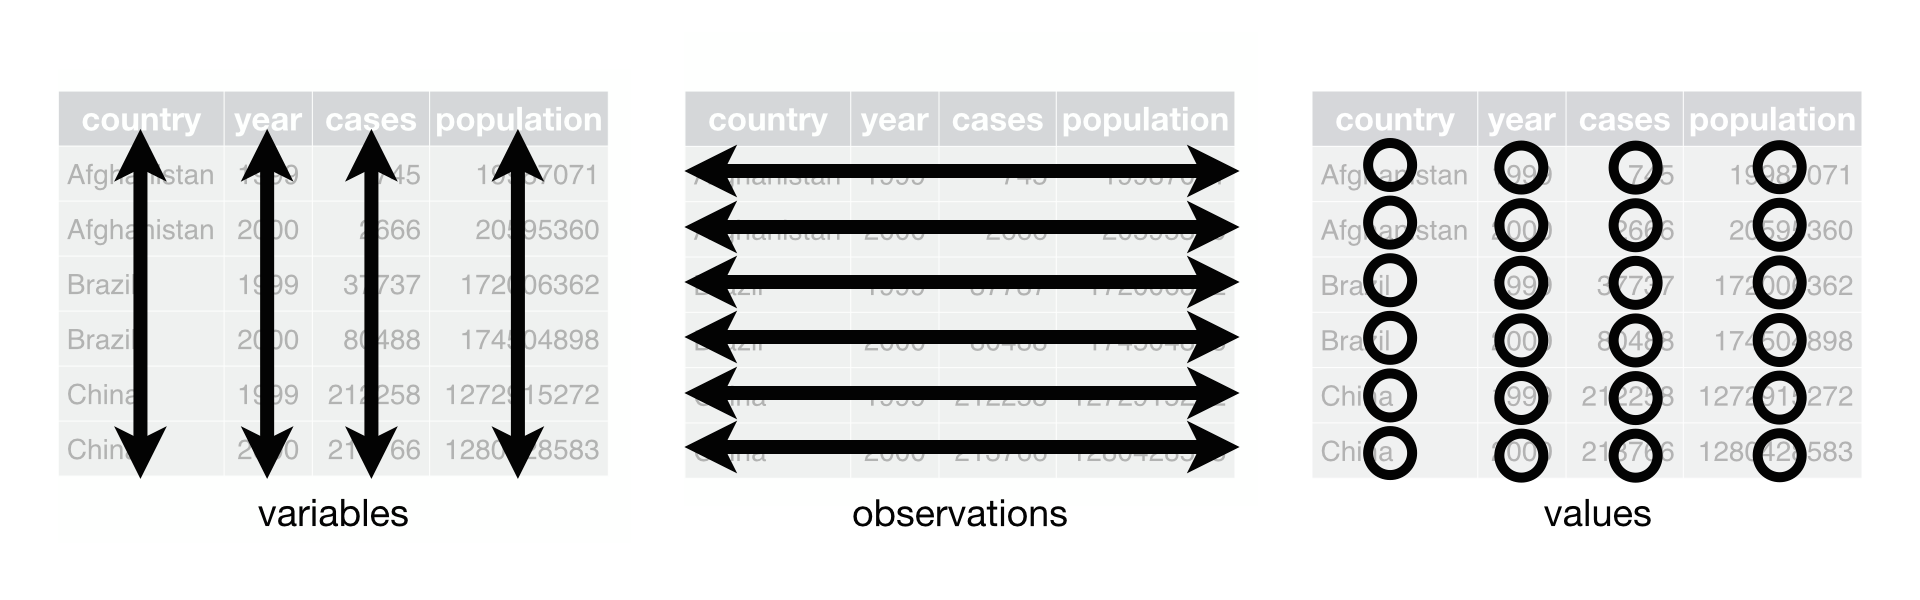
\includegraphics{images/tidy-1.png}

\end{center}

\end{frame}

\begin{frame}[fragile]{Why tidying a dataset ?}

\begin{center}
\begin{table}[t]

\caption{\label{tab:show1}Typical presentation dataset}
\centering
\begin{tabular}{l|r|r|r}
\hline
  & treatment\_a & treatment\_b & treatment\_c\\
\hline
John Smith & 13 & 20 & 21\\
\hline
Jane Doe & 11 & 16 & 16\\
\hline
Mary Johnson & 10 & 21 & 22\\
\hline
\end{tabular}
\end{table}
\end{center}

\begin{Shaded}
\begin{Highlighting}[]
\KeywordTok{boxplot}\NormalTok{(treatments)}
\end{Highlighting}
\end{Shaded}

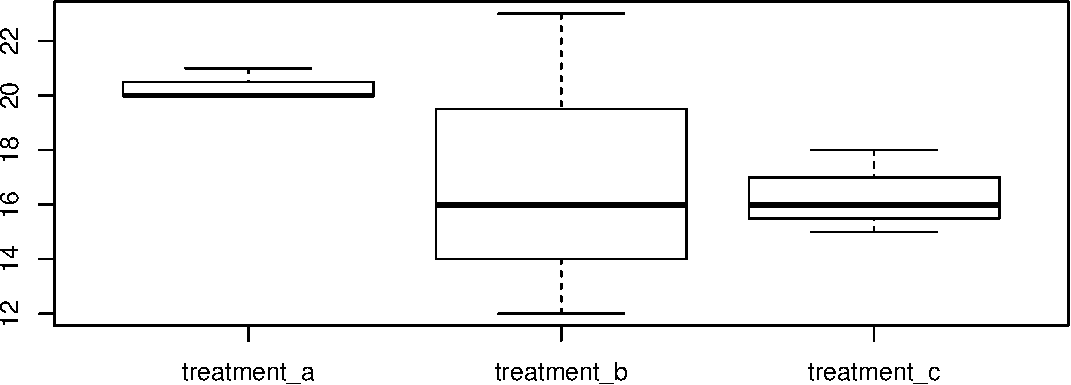
\includegraphics{tidyverse_28_03_files/figure-beamer/boxplot1-1.pdf}

\end{frame}

\begin{frame}[fragile]{Why tidying a dataset ?}

\begin{Shaded}
\begin{Highlighting}[]
\NormalTok{treatments.}\DecValTok{2}\NormalTok{ <-}\StringTok{ }\KeywordTok{t}\NormalTok{(treatments)}
\end{Highlighting}
\end{Shaded}

\begin{center}
\begin{table}[t]

\caption{\label{tab:unnamed-chunk-4}The same data but structured differently}
\centering
\begin{tabular}{l|r|r|r}
\hline
  & John Smith & Jane Doe & Mary Johnson\\
\hline
treatment\_a & 13 & 11 & 10\\
\hline
treatment\_b & 20 & 16 & 21\\
\hline
treatment\_c & 21 & 16 & 22\\
\hline
\end{tabular}
\end{table}
\end{center}

\begin{Shaded}
\begin{Highlighting}[]
\KeywordTok{boxplot}\NormalTok{(treatments.}\DecValTok{2}\NormalTok{)}
\end{Highlighting}
\end{Shaded}

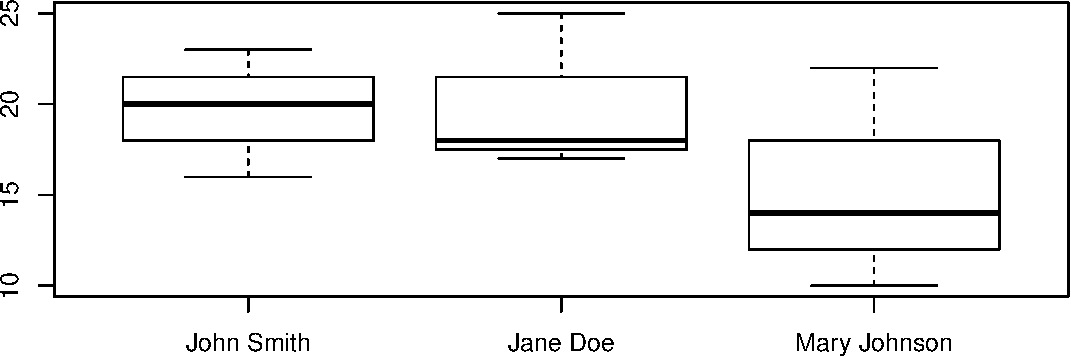
\includegraphics{tidyverse_28_03_files/figure-beamer/boxplot2-1.pdf}

\end{frame}

\begin{frame}[fragile]{Why tidying a dataset ?}

\begin{center}
\begin{table}[t]

\caption{\label{tab:unnamed-chunk-5}An exemple of a tidy dataset}
\centering
\begin{tabular}{l|l|r}
\hline
person & treatment & result\\
\hline
John Smith & treatment\_a & 13\\
\hline
Jane Doe & treatment\_a & 11\\
\hline
Mary Johnson & treatment\_a & 10\\
\hline
John Smith & treatment\_b & 20\\
\hline
Jane Doe & treatment\_b & 16\\
\hline
Mary Johnson & treatment\_b & 21\\
\hline
John Smith & treatment\_c & 21\\
\hline
Jane Doe & treatment\_c & 16\\
\hline
Mary Johnson & treatment\_c & 22\\
\hline
\end{tabular}
\end{table}
\end{center}

\begin{Shaded}
\begin{Highlighting}[]
\KeywordTok{boxplot}\NormalTok{(result}\OperatorTok{~}\NormalTok{treatment,}\DataTypeTok{data=}\NormalTok{treatments.}\DecValTok{3}\NormalTok{)}
\end{Highlighting}
\end{Shaded}

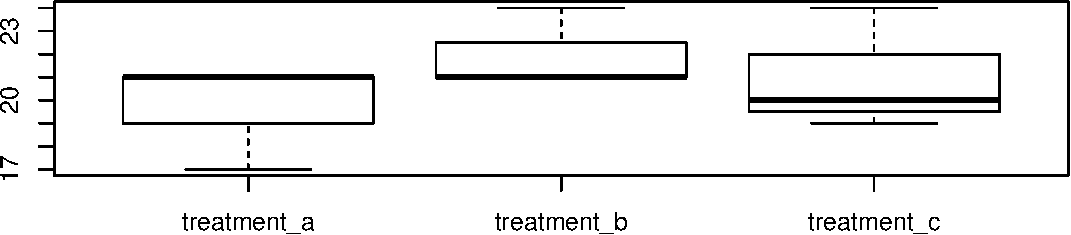
\includegraphics{tidyverse_28_03_files/figure-beamer/boxplot3-1.pdf}

\end{frame}

\begin{frame}[fragile]{Why tidying a dataset ?}

\begin{Shaded}
\begin{Highlighting}[]
\KeywordTok{boxplot}\NormalTok{(result}\OperatorTok{~}\NormalTok{person,}\DataTypeTok{data=}\NormalTok{treatments.}\DecValTok{3}\NormalTok{)}
\end{Highlighting}
\end{Shaded}

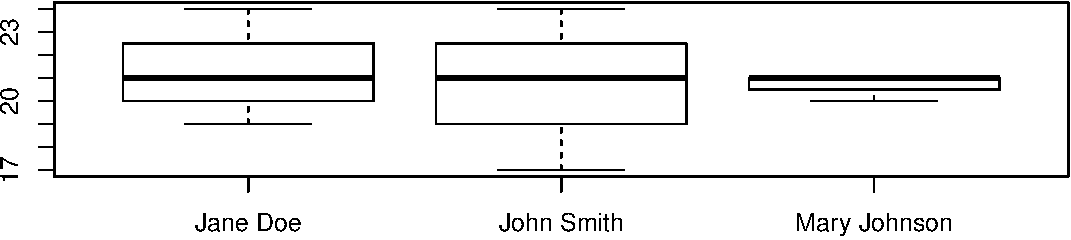
\includegraphics{tidyverse_28_03_files/figure-beamer/boxplot4-1.pdf}

\begin{Shaded}
\begin{Highlighting}[]
\KeywordTok{boxplot}\NormalTok{(result}\OperatorTok{~}\NormalTok{person}\OperatorTok{+}\NormalTok{treatment,}\DataTypeTok{data=}\NormalTok{treatments.}\DecValTok{3}\NormalTok{)}
\end{Highlighting}
\end{Shaded}

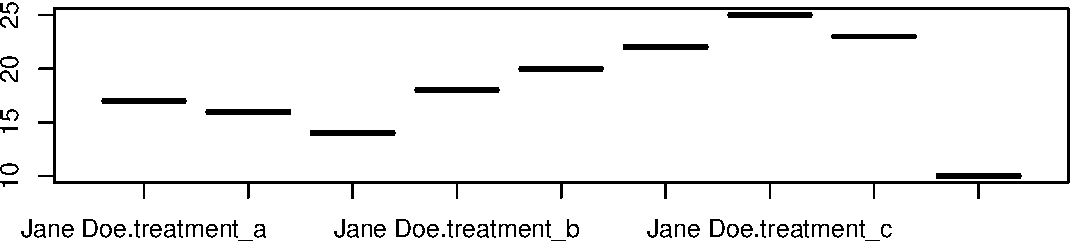
\includegraphics{tidyverse_28_03_files/figure-beamer/boxplot5-1.pdf}

\end{frame}

\section{Pipe and tibble}\label{pipe-and-tibble}

\begin{frame}[fragile]{Pipes}

\textbf{The pipe \%\textgreater{}\%:}

\begin{itemize}
\tightlist
\item
  Come from the \textbf{magrittr} package by Stefan Milton Bache.
\item
  Automatically loaded in tidyverse.
\item
  Equivalent to \texttt{\textbar{}} in \texttt{bash}
\end{itemize}

\begin{Shaded}
\begin{Highlighting}[]
\FunctionTok{cat}\NormalTok{ iris.tsv }\KeywordTok{|} \FunctionTok{cut}\NormalTok{ -f5 }\KeywordTok{|} \FunctionTok{sed} \StringTok{'s/^./\textbackslash{}U&/'} \KeywordTok{|} \FunctionTok{head}
\end{Highlighting}
\end{Shaded}

\begin{verbatim}
## Species
## Setosa
## Setosa
## Setosa
## Setosa
## Setosa
## Setosa
## Setosa
## Setosa
## Setosa
\end{verbatim}

\begin{Shaded}
\begin{Highlighting}[]
\KeywordTok{read_tsv}\NormalTok{(}\StringTok{"iris.tsv"}\NormalTok{,}\DataTypeTok{col_names =}\NormalTok{ F) }\OperatorTok\StringTok{ }\KeywordTok{pull}\NormalTok{(}\DecValTok{5}\NormalTok{) }\OperatorTok\StringTok{ }\KeywordTok{str_to_title}\NormalTok{() }\OperatorTok\StringTok{ }\NormalTok{head}
\end{Highlighting}
\end{Shaded}

\begin{verbatim}
## [1] "Species" "Setosa"  "Setosa"  "Setosa"  "Setosa"  "Setosa"
\end{verbatim}

\end{frame}

\begin{frame}[fragile]{Pipes vs no pipes : without pipe}

\begin{Shaded}
\begin{Highlighting}[]
\NormalTok{ex.dat <-}\StringTok{ }\KeywordTok{rnorm}\NormalTok{(}\DataTypeTok{n =} \DecValTok{1000}\NormalTok{,}\DataTypeTok{mean =} \DecValTok{5}\NormalTok{,}\DataTypeTok{sd=}\DecValTok{1}\NormalTok{)}
\NormalTok{sub.dat <-}\StringTok{ }\KeywordTok{sample}\NormalTok{(ex.dat,}\DataTypeTok{size =} \DecValTok{100}\NormalTok{,}\DataTypeTok{replace=}\NormalTok{F)}
\KeywordTok{hist}\NormalTok{(sub.dat)}
\end{Highlighting}
\end{Shaded}

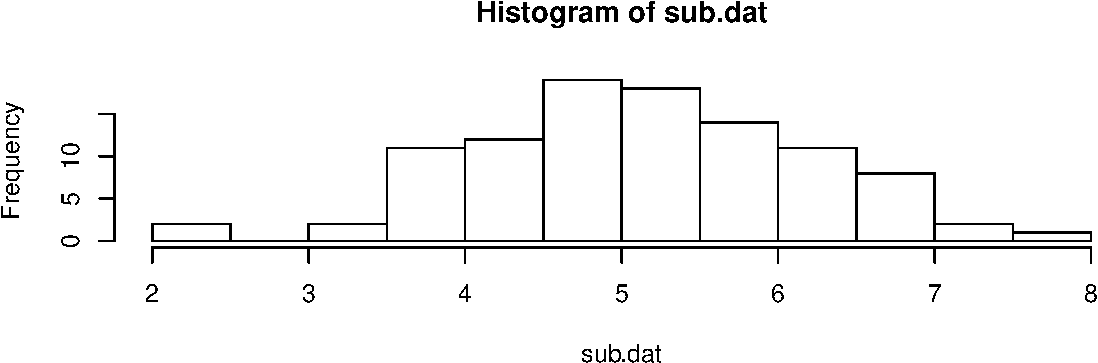
\includegraphics{tidyverse_28_03_files/figure-beamer/histo1-1.pdf}

\end{frame}

\begin{frame}[fragile]{Pipes vs no pipes : without pipe}

\begin{Shaded}
\begin{Highlighting}[]
\KeywordTok{hist}\NormalTok{(}\KeywordTok{sample}\NormalTok{(}\KeywordTok{rnorm}\NormalTok{(}\DataTypeTok{n =} \DecValTok{1000}\NormalTok{,}\DataTypeTok{mean =} \DecValTok{5}\NormalTok{,}\DataTypeTok{sd=}\DecValTok{1}\NormalTok{),}\DataTypeTok{size =} \DecValTok{100}\NormalTok{,}\DataTypeTok{replace=}\NormalTok{F))}
\end{Highlighting}
\end{Shaded}

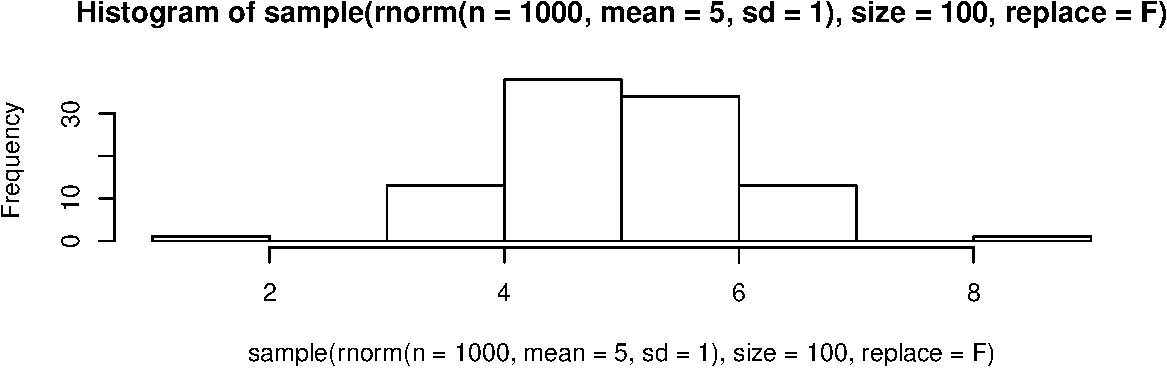
\includegraphics{tidyverse_28_03_files/figure-beamer/histo2-1.pdf}

\end{frame}

\begin{frame}[fragile]{Pipes vs no pipes : with pipe}

\begin{Shaded}
\begin{Highlighting}[]
\KeywordTok{rnorm}\NormalTok{(}\DataTypeTok{n =} \DecValTok{1000}\NormalTok{,}\DataTypeTok{mean =} \DecValTok{5}\NormalTok{,}\DataTypeTok{sd=}\DecValTok{1}\NormalTok{) }\OperatorTok
\StringTok{    }\KeywordTok{sample}\NormalTok{(}\DataTypeTok{size =} \DecValTok{100}\NormalTok{,}\DataTypeTok{replace=}\NormalTok{F) }\OperatorTok
\StringTok{    }\KeywordTok{hist}\NormalTok{()}
\end{Highlighting}
\end{Shaded}

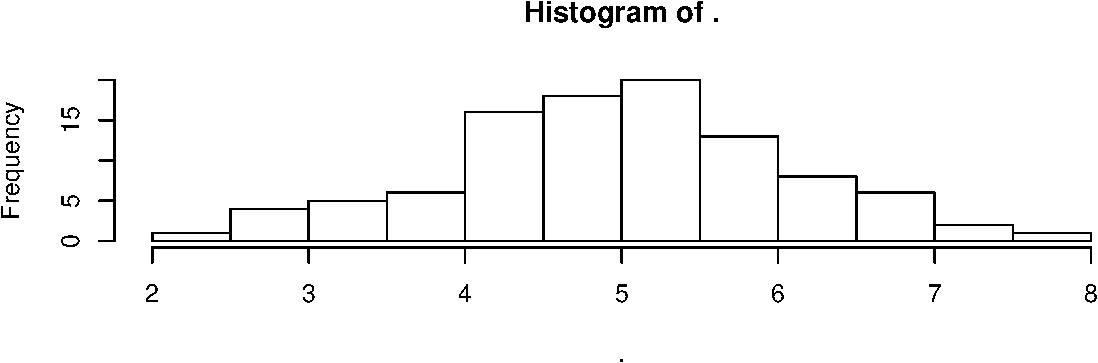
\includegraphics{tidyverse_28_03_files/figure-beamer/histo3-1.pdf}

\end{frame}

\begin{frame}[fragile]{Tibbles: \texttt{tibble::tibble}}

\begin{Shaded}
\begin{Highlighting}[]
\NormalTok{my.tibble <-}\StringTok{ }\KeywordTok{tibble}\NormalTok{(}
    \DataTypeTok{person =} \KeywordTok{c}\NormalTok{(}\StringTok{"John Smith"}\NormalTok{,}\StringTok{"Jane Doe"}\NormalTok{,}\StringTok{"Mary Johnson"}\NormalTok{),}
    \DataTypeTok{treatment_a =} \KeywordTok{sample}\NormalTok{(}\DecValTok{10}\OperatorTok{:}\DecValTok{25}\NormalTok{,}\DataTypeTok{size =} \DecValTok{3}\NormalTok{,}\DataTypeTok{replace =}\NormalTok{ T),}
    \DataTypeTok{treatment_b =} \KeywordTok{sample}\NormalTok{(}\DecValTok{10}\OperatorTok{:}\DecValTok{25}\NormalTok{,}\DataTypeTok{size =} \DecValTok{3}\NormalTok{,}\DataTypeTok{replace =}\NormalTok{ T),}
    \DataTypeTok{treatment_c =} \KeywordTok{sample}\NormalTok{(}\DecValTok{10}\OperatorTok{:}\DecValTok{25}\NormalTok{,}\DataTypeTok{size =} \DecValTok{3}\NormalTok{,}\DataTypeTok{replace =}\NormalTok{ T)}
\NormalTok{)}
\end{Highlighting}
\end{Shaded}

\begin{verbatim}
## # A tibble: 3 x 4
##   person       treatment_a treatment_b treatment_c
##   <chr>              <int>       <int>       <int>
## 1 John Smith            18          12          15
## 2 Jane Doe              17          15          17
## 3 Mary Johnson          14          14          15
\end{verbatim}

\end{frame}

\begin{frame}[fragile]{Tibbles: \texttt{tibble::tibble()}}

\textbf{Pros: }

\begin{itemize}
\tightlist
\item
  Cells can contain list and data.frame.
\item
  It never changes an input's type (i.e., no more
  \texttt{stringsAsFactors\ =\ FALSE}!).
\item
  Can use not valid R variable names (\texttt{:)}) as column names.
\item
  Refined print method that shows only the first 10 rows.
\end{itemize}

\textbf{Cons: }

\begin{itemize}
\tightlist
\item
  It never uses \texttt{row.names()}.

  \begin{itemize}
  \tightlist
  \item
    use \texttt{tibble::rownames\_to\_column()}.
  \end{itemize}
\end{itemize}

\begin{Shaded}
\begin{Highlighting}[]
\NormalTok{treatments }\OperatorTok\StringTok{ }\NormalTok{tibble}\OperatorTok{::}\KeywordTok{rownames_to_column}\NormalTok{(}\StringTok{"person"}\NormalTok{) }\OperatorTok
\StringTok{    }\KeywordTok{as_tibble}\NormalTok{() }\OperatorTok
\StringTok{    }\KeywordTok{rename}\NormalTok{(}\StringTok{`}\DataTypeTok{:)}\StringTok{`}\NormalTok{ =}\StringTok{ }\NormalTok{person)}
\end{Highlighting}
\end{Shaded}

\begin{verbatim}
## # A tibble: 3 x 4
##   `:)`         treatment_a treatment_b treatment_c
##   <chr>              <int>       <int>       <int>
## 1 John Smith            13          20          21
## 2 Jane Doe              11          16          16
## 3 Mary Johnson          10          21          22
\end{verbatim}

\end{frame}

\begin{frame}[fragile]{Split a dataset into multiples dataset using
\texttt{tidyr::nest()}}

\begin{Shaded}
\begin{Highlighting}[]
\NormalTok{my.tibble.split <-}\StringTok{ }\NormalTok{my.tibble }\OperatorTok\StringTok{ }\KeywordTok{group_by}\NormalTok{(person) }\OperatorTok\StringTok{ }\KeywordTok{nest}\NormalTok{(}\DataTypeTok{.key =}\NormalTok{ Data)}
\NormalTok{my.tibble.split}
\end{Highlighting}
\end{Shaded}

\begin{verbatim}
## # A tibble: 3 x 2
##   person       Data            
##   <chr>        <list>          
## 1 John Smith   <tibble [1 x 3]>
## 2 Jane Doe     <tibble [1 x 3]>
## 3 Mary Johnson <tibble [1 x 3]>
\end{verbatim}

\begin{Shaded}
\begin{Highlighting}[]
\NormalTok{my.tibble.split[[}\StringTok{"Data"}\NormalTok{]][[}\DecValTok{1}\NormalTok{]]}
\end{Highlighting}
\end{Shaded}

\begin{verbatim}
## # A tibble: 1 x 3
##   treatment_a treatment_b treatment_c
##         <int>       <int>       <int>
## 1          18          12          15
\end{verbatim}

\end{frame}

\begin{frame}[fragile]{Read/write tibbles: \texttt{readr::read\_*} /
\texttt{readr::write\_*}}

\Huge
\textbf{Read/write tibbles:} :

\begin{itemize}
\item
  \texttt{readr::read\_*}:

  \begin{itemize}
  \tightlist
  \item
    \texttt{read\_csv}: comma delimited files.
  \item
    \texttt{read\_csv2}: semi-colon delimited files.
  \item
    \texttt{read\_tsv}: tab delimited files.
  \item
    \texttt{read\_delim}: any delimiter.
  \end{itemize}
\item
  \texttt{readr::write\_*}:

  \begin{itemize}
  \tightlist
  \item
    \texttt{write\_csv}: comma delimited files.
  \item
    \texttt{write\_csv2}: semi-colon delimited files.
  \item
    \texttt{write\_tsv}: tab delimited files.
  \item
    \texttt{write\_delim}: any delimiter.
  \end{itemize}
\end{itemize}

\end{frame}

\begin{frame}[fragile]{Read/write tibbles: \texttt{readr::read\_*} /
\texttt{readr::write\_*}}

\begin{Shaded}
\begin{Highlighting}[]
\KeywordTok{read_tsv}\NormalTok{(}\StringTok{"iris.tsv"}\NormalTok{,}
         \DataTypeTok{col_types =} \KeywordTok{cols}\NormalTok{(}
            \DataTypeTok{Sepal.Length =} \KeywordTok{col_double}\NormalTok{(),}\DataTypeTok{Sepal.Width =} \KeywordTok{col_double}\NormalTok{(),}
            \DataTypeTok{Petal.Length =} \KeywordTok{col_double}\NormalTok{(),}\DataTypeTok{Petal.Width =} \KeywordTok{col_double}\NormalTok{(),}
            \DataTypeTok{Species =} \KeywordTok{col_character}\NormalTok{()}
\NormalTok{         )}
\NormalTok{    )}
\end{Highlighting}
\end{Shaded}

\begin{verbatim}
## # A tibble: 150 x 5
##    Sepal.Length Sepal.Width Petal.Length Petal.Width Species
##           <dbl>       <dbl>        <dbl>       <dbl> <chr>  
##  1          5.1         3.5          1.4         0.2 setosa 
##  2          4.9         3            1.4         0.2 setosa 
##  3          4.7         3.2          1.3         0.2 setosa 
##  4          4.6         3.1          1.5         0.2 setosa 
##  5          5           3.6          1.4         0.2 setosa 
##  6          5.4         3.9          1.7         0.4 setosa 
##  7          4.6         3.4          1.4         0.3 setosa 
##  8          5           3.4          1.5         0.2 setosa 
##  9          4.4         2.9          1.4         0.2 setosa 
## 10          4.9         3.1          1.5         0.1 setosa 
## # ... with 140 more rows
\end{verbatim}

\end{frame}

\section{Tidying dataset}\label{tidying-dataset}

\begin{frame}[fragile]{Using \texttt{tidyr} to reshape data}

Use \texttt{tidyr::gather()} and \texttt{tidyr::spread()} to reorganize
the value.

\begin{Shaded}
\begin{Highlighting}[]
\NormalTok{treatments }\OperatorTok\StringTok{ }\NormalTok{tibble}\OperatorTok{::}\KeywordTok{rownames_to_column}\NormalTok{(}\StringTok{"person"}\NormalTok{) }\OperatorTok
\StringTok{    }\NormalTok{tidyr}\OperatorTok{::}\KeywordTok{gather}\NormalTok{(}\DataTypeTok{key=}\StringTok{"treatment"}\NormalTok{,}\DataTypeTok{value =} \StringTok{"result"}\NormalTok{,}\OperatorTok{-}\NormalTok{person)}
\end{Highlighting}
\end{Shaded}

\begin{verbatim}
##         person   treatment result
## 1   John Smith treatment_a     13
## 2     Jane Doe treatment_a     11
## 3 Mary Johnson treatment_a     10
## 4   John Smith treatment_b     20
## 5     Jane Doe treatment_b     16
## 6 Mary Johnson treatment_b     21
## 7   John Smith treatment_c     21
## 8     Jane Doe treatment_c     16
## 9 Mary Johnson treatment_c     22
\end{verbatim}

\begin{Shaded}
\begin{Highlighting}[]
\NormalTok{treatment.}\DecValTok{3} \OperatorTok\StringTok{ }\KeywordTok{spread}\NormalTok{(}\DataTypeTok{key =} \StringTok{"treatment"}\NormalTok{,}\DataTypeTok{value =} \StringTok{"result"}\NormalTok{)}
\end{Highlighting}
\end{Shaded}

\begin{verbatim}
##         person treatment_a treatment_b treatment_c
## 1     Jane Doe          11          16          16
## 2   John Smith          13          20          21
## 3 Mary Johnson          10          21          22
\end{verbatim}

\end{frame}

\begin{frame}[fragile]{Using \texttt{tidyr} to reshape data}

\begin{Shaded}
\begin{Highlighting}[]
\NormalTok{treatment.}\DecValTok{3} \OperatorTok\StringTok{ }\KeywordTok{separate}\NormalTok{(person,}\DataTypeTok{into =} \KeywordTok{c}\NormalTok{(}\StringTok{"First Name"}\NormalTok{,}\StringTok{"Last Name"}\NormalTok{),}\DataTypeTok{sep=}\StringTok{" "}\NormalTok{)}
\end{Highlighting}
\end{Shaded}

\begin{verbatim}
##   First Name Last Name   treatment result
## 1       John     Smith treatment_a     13
## 2       Jane       Doe treatment_a     11
## 3       Mary   Johnson treatment_a     10
## 4       John     Smith treatment_b     20
## 5       Jane       Doe treatment_b     16
## 6       Mary   Johnson treatment_b     21
## 7       John     Smith treatment_c     21
## 8       Jane       Doe treatment_c     16
## 9       Mary   Johnson treatment_c     22
\end{verbatim}

\end{frame}

\section{\texorpdfstring{Manipulate a dataset using
\texttt{dplyr}}{Manipulate a dataset using dplyr}}\label{manipulate-a-dataset-using-dplyr}

\begin{frame}[fragile]{\texttt{dplyr}}

\textbf{\texttt{dplyr}:}

\begin{itemize}
\tightlist
\item
  Manipulate variables.
\item
  Manipulate observations.
\item
  Group / summarise observations.
\end{itemize}

\begin{center}
\begin{table}[t]

\caption{\label{tab:unnamed-chunk-20}iris dataset}
\centering
\begin{tabular}{r|r|r|r|l}
\hline
Sepal.Length & Sepal.Width & Petal.Length & Petal.Width & Species\\
\hline
5.1 & 3.5 & 1.4 & 0.2 & setosa\\
\hline
4.9 & 3.0 & 1.4 & 0.2 & setosa\\
\hline
4.7 & 3.2 & 1.3 & 0.2 & setosa\\
\hline
4.6 & 3.1 & 1.5 & 0.2 & setosa\\
\hline
5.0 & 3.6 & 1.4 & 0.2 & setosa\\
\hline
5.4 & 3.9 & 1.7 & 0.4 & setosa\\
\hline
\end{tabular}
\end{table}
\end{center}

\begin{block}{iris dataset}

The famous (Fisher's or Anderson's) iris data set gives the measurements
in centimeters of the variables sepal length and width and petal length
and width, respectively, for 50 flowers from each of 3 species of iris.
The species are Iris setosa, versicolor, and virginica. (from ?iris)

\end{block}

\end{frame}

\begin{frame}[fragile]{Manipulate \textbf{variables} using
\texttt{dplyr::select()}}

\begin{Shaded}
\begin{Highlighting}[]
\NormalTok{iris.tbl }\OperatorTok\StringTok{ }\KeywordTok{select}\NormalTok{(}\DecValTok{1}\OperatorTok{:}\DecValTok{3}\NormalTok{)}
\NormalTok{iris.tbl }\OperatorTok\StringTok{ }\KeywordTok{select}\NormalTok{(Sepal.Length,Sepal.Width,Petal.Length)}
\NormalTok{iris.tbl }\OperatorTok\StringTok{ }\KeywordTok{select}\NormalTok{(Sepal.Length}\OperatorTok{:}\NormalTok{Petal.Length)}
\NormalTok{iris.tbl }\OperatorTok\StringTok{ }\KeywordTok{select}\NormalTok{(}\OperatorTok{-}\NormalTok{Petal.Width,}\OperatorTok{-}\NormalTok{Species)}
\end{Highlighting}
\end{Shaded}

\begin{verbatim}
## # A tibble: 150 x 3
##    Sepal.Length Sepal.Width Petal.Length
##           <dbl>       <dbl>        <dbl>
##  1          5.1         3.5          1.4
##  2          4.9         3            1.4
##  3          4.7         3.2          1.3
##  4          4.6         3.1          1.5
##  5          5           3.6          1.4
##  6          5.4         3.9          1.7
##  7          4.6         3.4          1.4
##  8          5           3.4          1.5
##  9          4.4         2.9          1.4
## 10          4.9         3.1          1.5
## # ... with 140 more rows
\end{verbatim}

\end{frame}

\begin{frame}[fragile]{Manipulate \textbf{variables} using
\texttt{dplyr::select()}}

\begin{Shaded}
\begin{Highlighting}[]
\NormalTok{iris.tbl }\OperatorTok\StringTok{ }\KeywordTok{select}\NormalTok{(}\KeywordTok{starts_with}\NormalTok{(}\StringTok{"Petal"}\NormalTok{))}
\end{Highlighting}
\end{Shaded}

\begin{verbatim}
## # A tibble: 150 x 2
##    Petal.Length Petal.Width
##           <dbl>       <dbl>
##  1          1.4         0.2
##  2          1.4         0.2
##  3          1.3         0.2
##  4          1.5         0.2
##  5          1.4         0.2
##  6          1.7         0.4
##  7          1.4         0.3
##  8          1.5         0.2
##  9          1.4         0.2
## 10          1.5         0.1
## # ... with 140 more rows
\end{verbatim}

\end{frame}

\begin{frame}[fragile]{Manipulate \textbf{variables} using
\texttt{dplyr::pull()}}

\begin{Shaded}
\begin{Highlighting}[]
\NormalTok{iris.tbl }\OperatorTok\StringTok{ }\KeywordTok{select}\NormalTok{(Sepal.Length)}
\end{Highlighting}
\end{Shaded}

\begin{verbatim}
## # A tibble: 150 x 1
##   Sepal.Length
##          <dbl>
## 1          5.1
## 2          4.9
## 3          4.7
## 4          4.6
## 5          5  
## # ... with 145 more rows
\end{verbatim}

\begin{Shaded}
\begin{Highlighting}[]
\NormalTok{iris.tbl }\OperatorTok\StringTok{ }\KeywordTok{pull}\NormalTok{(Sepal.Length)}
\end{Highlighting}
\end{Shaded}

\begin{verbatim}
## [1] 5.1 4.9 4.7 4.6 5.0
\end{verbatim}

\end{frame}

\begin{frame}[fragile]{Modify \textbf{variables} using
\texttt{dplyr::mutate()}}

\begin{Shaded}
\begin{Highlighting}[]
\NormalTok{iris.tbl }\OperatorTok
\StringTok{    }\KeywordTok{mutate}\NormalTok{(}\DataTypeTok{Petal.Length =} 
\NormalTok{               scales}\OperatorTok{::}\KeywordTok{percent}\NormalTok{(Petal.Length}\OperatorTok{/}\KeywordTok{max}\NormalTok{(Petal.Length))}
\NormalTok{           )}
\end{Highlighting}
\end{Shaded}

\begin{verbatim}
## # A tibble: 150 x 5
##    Sepal.Length Sepal.Width Petal.Length Petal.Width Species
##           <dbl>       <dbl> <chr>              <dbl> <fct>  
##  1          5.1         3.5 20.3%                0.2 setosa 
##  2          4.9         3   20.3%                0.2 setosa 
##  3          4.7         3.2 18.8%                0.2 setosa 
##  4          4.6         3.1 21.7%                0.2 setosa 
##  5          5           3.6 20.3%                0.2 setosa 
##  6          5.4         3.9 24.6%                0.4 setosa 
##  7          4.6         3.4 20.3%                0.3 setosa 
##  8          5           3.4 21.7%                0.2 setosa 
##  9          4.4         2.9 20.3%                0.2 setosa 
## 10          4.9         3.1 21.7%                0.1 setosa 
## # ... with 140 more rows
\end{verbatim}

\end{frame}

\begin{frame}[fragile]{Create \textbf{variables} using
\texttt{dplyr::mutate()}}

\begin{Shaded}
\begin{Highlighting}[]
\NormalTok{iris.tbl }\OperatorTok
\StringTok{    }\CommentTok{#Case 1}
\StringTok{    }\KeywordTok{mutate}\NormalTok{(}\DataTypeTok{Size =}\NormalTok{ dplyr}\OperatorTok{::}\KeywordTok{case_when}\NormalTok{(}
\NormalTok{            Petal.Length }\OperatorTok{>=}\StringTok{ }\DecValTok{4} \OperatorTok{&}\StringTok{ }\NormalTok{Petal.Width }\OperatorTok{>=}\StringTok{ }\FloatTok{1.3} \OperatorTok{~}\StringTok{ "Big"}\NormalTok{,}
\NormalTok{            Petal.Length }\OperatorTok{<}\StringTok{ }\DecValTok{4} \OperatorTok{&}\StringTok{ }\NormalTok{Petal.Width }\OperatorTok{<}\StringTok{ }\FloatTok{1.3} \OperatorTok{~}\StringTok{ "Small"}
\NormalTok{        )}
\NormalTok{    ) }\OperatorTok
\StringTok{    }\CommentTok{#Case 2}
\StringTok{    }\KeywordTok{mutate}\NormalTok{(}\DataTypeTok{Ratio_Petal_Sepal_width =}\NormalTok{ Petal.Width}\OperatorTok{/}\NormalTok{Sepal.Width)}
\end{Highlighting}
\end{Shaded}

\begin{verbatim}
## # A tibble: 3 x 7
##   Ratio_Petal_Sep~ Size  Sepal.Length Sepal.Width Petal.Length Petal.Width
##              <dbl> <chr>        <dbl>       <dbl>        <dbl>       <dbl>
## 1           0.0571 Small          5.1         3.5          1.4         0.2
## 2           0.0667 Small          4.9         3            1.4         0.2
## 3           0.0625 Small          4.7         3.2          1.3         0.2
## # ... with 1 more variable: Species <fct>
\end{verbatim}

other functions:

\begin{itemize}
\tightlist
\item
  \texttt{dplyr::mutate\_all()}: Apply a function to every columns.
\item
  \texttt{dplyr::mutate\_at()}: Apply a function to specific column.
\end{itemize}

\end{frame}

\begin{frame}[fragile]{Mutating joins using \texttt{dplyr::*\_join()}}

\begin{Shaded}
\begin{Highlighting}[]
\NormalTok{iris.meta <-}\StringTok{ }\KeywordTok{tibble}\NormalTok{(}
    \DataTypeTok{Species =} \KeywordTok{factor}\NormalTok{(}\KeywordTok{c}\NormalTok{(}\StringTok{"setosa"}\NormalTok{,}\StringTok{"versicolor"}\NormalTok{,}\StringTok{"virginica"}\NormalTok{)),}
    \DataTypeTok{Colony =} \KeywordTok{c}\NormalTok{(}\StringTok{"A"}\NormalTok{,}\StringTok{"A"}\NormalTok{,}\StringTok{"B"}\NormalTok{) ,}
    \DataTypeTok{Ploidy =} \KeywordTok{c}\NormalTok{(}\StringTok{"diploid"}\NormalTok{,}\StringTok{"hexaploid"}\NormalTok{,}\StringTok{"tetraploid"}\NormalTok{),}
    \StringTok{`}\DataTypeTok{Common name}\StringTok{`}\NormalTok{ =}\StringTok{ }\KeywordTok{c}\NormalTok{(}\StringTok{"Beachhead iris"}\NormalTok{,}\StringTok{"Harlequin blueflag"}\NormalTok{,}\StringTok{"Virginia iris"}\NormalTok{)}
\NormalTok{)}
\end{Highlighting}
\end{Shaded}

\begin{table}[t]

\caption{\label{tab:unnamed-chunk-32}Metadata for iris dataset}
\centering
\begin{tabular}{l|l|l|l}
\hline
Species & Colony & Ploidy & Common name\\
\hline
setosa & A & diploid & Beachhead iris\\
\hline
versicolor & A & hexaploid & Harlequin blueflag\\
\hline
virginica & B & tetraploid & Virginia iris\\
\hline
\end{tabular}
\end{table}

\end{frame}

\begin{frame}[fragile]{Arrange dataset using \texttt{dplyr::arrange()}}

\begin{Shaded}
\begin{Highlighting}[]
\NormalTok{iris.tbl }\OperatorTok\StringTok{ }\KeywordTok{arrange}\NormalTok{(Petal.Length) }\OperatorTok\StringTok{ }\KeywordTok{slice}\NormalTok{(}\DecValTok{1}\OperatorTok{:}\DecValTok{5}\NormalTok{)}
\end{Highlighting}
\end{Shaded}

\begin{verbatim}
## # A tibble: 5 x 5
##   Sepal.Length Sepal.Width Petal.Length Petal.Width Species
##          <dbl>       <dbl>        <dbl>       <dbl> <fct>  
## 1          4.6         3.6          1           0.2 setosa 
## 2          4.3         3            1.1         0.1 setosa 
## 3          5.8         4            1.2         0.2 setosa 
## 4          5           3.2          1.2         0.2 setosa 
## 5          4.7         3.2          1.3         0.2 setosa
\end{verbatim}

\begin{Shaded}
\begin{Highlighting}[]
\NormalTok{iris.tbl }\OperatorTok\StringTok{ }\KeywordTok{filter}\NormalTok{(}\KeywordTok{min_rank}\NormalTok{(Petal.Length) }\OperatorTok{<=}\StringTok{ }\DecValTok{5}\NormalTok{)}
\NormalTok{iris.tbl }\OperatorTok\StringTok{ }\KeywordTok{top_n}\NormalTok{(}\OperatorTok{-}\DecValTok{5}\NormalTok{,Petal.Length) }
\end{Highlighting}
\end{Shaded}

Use \texttt{desc()} to order by high to low.

\end{frame}

\begin{frame}[fragile]{Manipulate \textbf{observations} using
\texttt{dplyr::filter()}}

\begin{Shaded}
\begin{Highlighting}[]
\NormalTok{iris.tbl }\OperatorTok\StringTok{ }\KeywordTok{filter}\NormalTok{(Sepal.Length }\OperatorTok{<}\StringTok{ }\DecValTok{7}\NormalTok{) }\OperatorTok\StringTok{ }\KeywordTok{slice}\NormalTok{(}\DecValTok{1}\OperatorTok{:}\DecValTok{5}\NormalTok{)}
\end{Highlighting}
\end{Shaded}

\begin{verbatim}
## # A tibble: 5 x 5
##   Sepal.Length Sepal.Width Petal.Length Petal.Width Species
##          <dbl>       <dbl>        <dbl>       <dbl> <fct>  
## 1          5.1         3.5          1.4         0.2 setosa 
## 2          4.9         3            1.4         0.2 setosa 
## 3          4.7         3.2          1.3         0.2 setosa 
## 4          4.6         3.1          1.5         0.2 setosa 
## 5          5           3.6          1.4         0.2 setosa
\end{verbatim}

\begin{Shaded}
\begin{Highlighting}[]
\NormalTok{iris.tbl }\OperatorTok\StringTok{ }\KeywordTok{filter}\NormalTok{(Species }\OperatorTok{==}\StringTok{  "setosa"}\NormalTok{) }\OperatorTok\StringTok{ }\KeywordTok{slice}\NormalTok{(}\DecValTok{1}\OperatorTok{:}\DecValTok{5}\NormalTok{)}
\end{Highlighting}
\end{Shaded}

\begin{verbatim}
## # A tibble: 5 x 5
##   Sepal.Length Sepal.Width Petal.Length Petal.Width Species
##          <dbl>       <dbl>        <dbl>       <dbl> <fct>  
## 1          5.1         3.5          1.4         0.2 setosa 
## 2          4.9         3            1.4         0.2 setosa 
## 3          4.7         3.2          1.3         0.2 setosa 
## 4          4.6         3.1          1.5         0.2 setosa 
## 5          5           3.6          1.4         0.2 setosa
\end{verbatim}

\end{frame}

\begin{frame}[fragile]{Manipulate \textbf{observations} using
\texttt{dplyr::filter()}}

\begin{Shaded}
\begin{Highlighting}[]
\NormalTok{iris.tbl }\OperatorTok
\StringTok{    }\KeywordTok{filter}\NormalTok{(Sepal.Length }\OperatorTok{<}\StringTok{ }\DecValTok{7}\NormalTok{) }\OperatorTok
\StringTok{    }\KeywordTok{filter}\NormalTok{(Species }\OperatorTok{==}\StringTok{  "setosa"}\NormalTok{) }\OperatorTok\StringTok{ }\KeywordTok{slice}\NormalTok{(}\DecValTok{1}\OperatorTok{:}\DecValTok{5}\NormalTok{)}
\end{Highlighting}
\end{Shaded}

\begin{verbatim}
## # A tibble: 5 x 5
##   Sepal.Length Sepal.Width Petal.Length Petal.Width Species
##          <dbl>       <dbl>        <dbl>       <dbl> <fct>  
## 1          5.1         3.5          1.4         0.2 setosa 
## 2          4.9         3            1.4         0.2 setosa 
## 3          4.7         3.2          1.3         0.2 setosa 
## 4          4.6         3.1          1.5         0.2 setosa 
## 5          5           3.6          1.4         0.2 setosa
\end{verbatim}

\begin{Shaded}
\begin{Highlighting}[]
\NormalTok{iris.tbl }\OperatorTok
\StringTok{    }\KeywordTok{filter}\NormalTok{(Sepal.Length }\OperatorTok{<}\StringTok{ }\DecValTok{7} \OperatorTok{&}\StringTok{ }\NormalTok{Species }\OperatorTok{==}\StringTok{  "setosa"}\NormalTok{) }\OperatorTok\StringTok{ }\KeywordTok{slice}\NormalTok{(}\DecValTok{1}\OperatorTok{:}\DecValTok{5}\NormalTok{)}

\NormalTok{iris.tbl }\OperatorTok
\StringTok{    }\KeywordTok{filter}\NormalTok{(Sepal.Length }\OperatorTok{<}\StringTok{ }\DecValTok{7}\NormalTok{,Species }\OperatorTok{==}\StringTok{  "setosa"}\NormalTok{) }\OperatorTok\StringTok{ }\KeywordTok{slice}\NormalTok{(}\DecValTok{1}\OperatorTok{:}\DecValTok{5}\NormalTok{)}
\end{Highlighting}
\end{Shaded}

\end{frame}

\begin{frame}[fragile]{\textbf{Summarise} observations using
\texttt{dplyr::summarise()}}

\begin{Shaded}
\begin{Highlighting}[]
\NormalTok{iris.tbl }\OperatorTok\StringTok{ }\KeywordTok{summarise}\NormalTok{(}\DataTypeTok{mean =} \KeywordTok{mean}\NormalTok{(Petal.Length), }\DataTypeTok{sd =} \KeywordTok{sd}\NormalTok{(Petal.Length))}
\end{Highlighting}
\end{Shaded}

\begin{verbatim}
## # A tibble: 1 x 2
##    mean    sd
##   <dbl> <dbl>
## 1  3.76  1.77
\end{verbatim}

\begin{Shaded}
\begin{Highlighting}[]
\NormalTok{iris.tbl }\OperatorTok\StringTok{ }\KeywordTok{select}\NormalTok{(}\OperatorTok{-}\NormalTok{Species) }\OperatorTok\KeywordTok{summarise_all}\NormalTok{(mean)}
\end{Highlighting}
\end{Shaded}

\begin{verbatim}
## # A tibble: 1 x 4
##   Sepal.Length Sepal.Width Petal.Length Petal.Width
##          <dbl>       <dbl>        <dbl>       <dbl>
## 1         5.84        3.06         3.76        1.20
\end{verbatim}

\begin{Shaded}
\begin{Highlighting}[]
\NormalTok{iris.tbl }\OperatorTok\StringTok{ }\KeywordTok{summarise}\NormalTok{(}\DataTypeTok{n =} \KeywordTok{n}\NormalTok{())}
\end{Highlighting}
\end{Shaded}

\begin{verbatim}
## # A tibble: 1 x 1
##       n
##   <int>
## 1   150
\end{verbatim}

\end{frame}

\begin{frame}[fragile]{\textbf{Summarise} observations using
\texttt{dplyr::group\_by()}}

\begin{Shaded}
\begin{Highlighting}[]
\NormalTok{iris.tbl }\OperatorTok\StringTok{ }\KeywordTok{group_by}\NormalTok{(Species) }\OperatorTok\StringTok{ }\KeywordTok{summarise}\NormalTok{(}\DataTypeTok{mean =} \KeywordTok{mean}\NormalTok{(Petal.Length), }\DataTypeTok{sd =} \KeywordTok{sd}\NormalTok{(Petal.Length))}
\end{Highlighting}
\end{Shaded}

\begin{verbatim}
## # A tibble: 3 x 3
##   Species     mean    sd
##   <fct>      <dbl> <dbl>
## 1 setosa      1.46 0.174
## 2 versicolor  4.26 0.470
## 3 virginica   5.55 0.552
\end{verbatim}

\begin{Shaded}
\begin{Highlighting}[]
\NormalTok{iris.tbl }\OperatorTok\StringTok{ }\KeywordTok{group_by}\NormalTok{(Species) }\OperatorTok\StringTok{ }\KeywordTok{summarise}\NormalTok{(}\DataTypeTok{n =} \KeywordTok{n}\NormalTok{())}
\end{Highlighting}
\end{Shaded}

\begin{verbatim}
## # A tibble: 3 x 2
##   Species        n
##   <fct>      <int>
## 1 setosa        50
## 2 versicolor    50
## 3 virginica     50
\end{verbatim}

\begin{Shaded}
\begin{Highlighting}[]
\NormalTok{iris.tbl }\OperatorTok\StringTok{ }\KeywordTok{group_by}\NormalTok{(Species) }\OperatorTok\StringTok{ }\KeywordTok{tally}\NormalTok{()}
\NormalTok{iris.tbl }\OperatorTok\StringTok{ }\KeywordTok{count}\NormalTok{(Species)}
\end{Highlighting}
\end{Shaded}

\end{frame}

\begin{frame}[fragile]{\textbf{Summarise} observations using
\texttt{dplyr::group\_by()}}

\begin{Shaded}
\begin{Highlighting}[]
\NormalTok{iris.tbl }\OperatorTok\StringTok{ }\KeywordTok{group_by}\NormalTok{(Species) }\OperatorTok\StringTok{ }\KeywordTok{filter}\NormalTok{(Petal.Length }\OperatorTok{>=}\StringTok{ }\KeywordTok{max}\NormalTok{(Petal.Length))}
\end{Highlighting}
\end{Shaded}

\begin{verbatim}
## # A tibble: 4 x 5
## # Groups:   Species [3]
##   Sepal.Length Sepal.Width Petal.Length Petal.Width Species   
##          <dbl>       <dbl>        <dbl>       <dbl> <fct>     
## 1          4.8         3.4          1.9         0.2 setosa    
## 2          5.1         3.8          1.9         0.4 setosa    
## 3          6           2.7          5.1         1.6 versicolor
## 4          7.7         2.6          6.9         2.3 virginica
\end{verbatim}

\begin{Shaded}
\begin{Highlighting}[]
\NormalTok{iris.tbl }\OperatorTok\StringTok{ }\KeywordTok{group_by}\NormalTok{(Species) }\OperatorTok\StringTok{ }\KeywordTok{top_n}\NormalTok{(}\DecValTok{1}\NormalTok{,Petal.Length)}
\end{Highlighting}
\end{Shaded}

\begin{verbatim}
## # A tibble: 4 x 5
## # Groups:   Species [3]
##   Sepal.Length Sepal.Width Petal.Length Petal.Width Species   
##          <dbl>       <dbl>        <dbl>       <dbl> <fct>     
## 1          4.8         3.4          1.9         0.2 setosa    
## 2          5.1         3.8          1.9         0.4 setosa    
## 3          6           2.7          5.1         1.6 versicolor
## 4          7.7         2.6          6.9         2.3 virginica
\end{verbatim}

\end{frame}

\begin{frame}[fragile]{Inner join}

\textbf{Inner join:} return all rows from \texttt{x} where there are
matching values in \texttt{y}, and all columns from \texttt{x} and
\texttt{y}. If there are multiple matches between \texttt{x} and
\texttt{y}, all combination of the matches are returned.

\begin{center}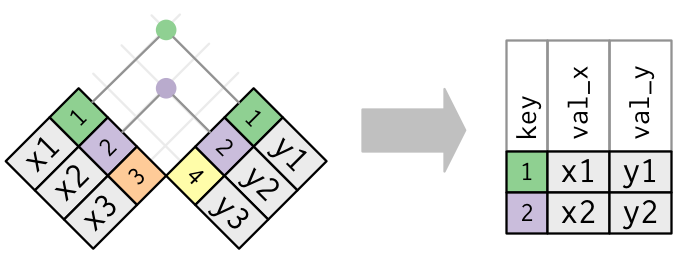
\includegraphics[width=0.4\linewidth]{images/join-inner} \end{center}

\small

\begin{Shaded}
\begin{Highlighting}[]
\NormalTok{iris.meta.nosetosa <-}\StringTok{ }\NormalTok{iris.meta }\OperatorTok\StringTok{ }\KeywordTok{filter}\NormalTok{(Species }\OperatorTok{!=}\StringTok{"setosa"}\NormalTok{)}
\NormalTok{iris.tbl }\OperatorTok\StringTok{ }\KeywordTok{inner_join}\NormalTok{(iris.meta.nosetosa,}\DataTypeTok{by =} \StringTok{"Species"}\NormalTok{) }\OperatorTok\StringTok{ }\KeywordTok{print}\NormalTok{(}\DataTypeTok{n=}\DecValTok{5}\NormalTok{)}
\end{Highlighting}
\end{Shaded}

\begin{verbatim}
## # A tibble: 100 x 8
##   Sepal.Length Sepal.Width Petal.Length Petal.Width Species Colony Ploidy
##          <dbl>       <dbl>        <dbl>       <dbl> <fct>   <chr>  <chr> 
## 1          7           3.2          4.7         1.4 versic~ A      hexap~
## 2          6.4         3.2          4.5         1.5 versic~ A      hexap~
## 3          6.9         3.1          4.9         1.5 versic~ A      hexap~
## 4          5.5         2.3          4           1.3 versic~ A      hexap~
## 5          6.5         2.8          4.6         1.5 versic~ A      hexap~
## # ... with 95 more rows, and 1 more variable: `Common name` <chr>
\end{verbatim}

\end{frame}

\begin{frame}[fragile]{Outer joins}

\begin{itemize}
\tightlist
\item
  A \textbf{left join} keeps all observations in \texttt{x}.
\item
  A \textbf{right join} keeps all observations in \texttt{y}.
\item
  A \textbf{full join} keeps all observations in \texttt{x} and
  \texttt{y}.
\end{itemize}

\begin{center}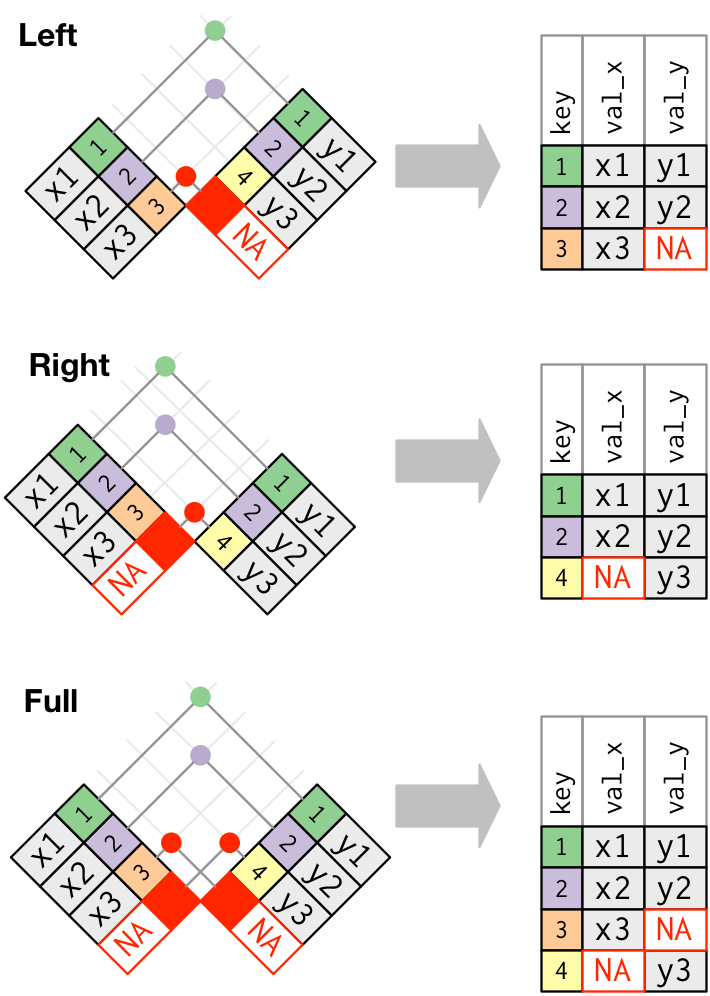
\includegraphics[width=0.35\linewidth]{images/join-outer} \end{center}

\end{frame}

\begin{frame}[fragile]{Outer joins}

\small
\textbf{left join:}

\begin{Shaded}
\begin{Highlighting}[]
\NormalTok{iris.meta.nosetosa <-}\StringTok{ }\NormalTok{iris.meta }\OperatorTok\StringTok{ }\KeywordTok{filter}\NormalTok{(Species }\OperatorTok{!=}\StringTok{"setosa"}\NormalTok{)}
\NormalTok{iris.tbl }\OperatorTok\StringTok{ }\KeywordTok{left_join}\NormalTok{(iris.meta.nosetosa,}\DataTypeTok{by =} \StringTok{"Species"}\NormalTok{) }\OperatorTok\StringTok{ }\KeywordTok{print}\NormalTok{(}\DataTypeTok{n=}\DecValTok{5}\NormalTok{)}
\end{Highlighting}
\end{Shaded}

\begin{verbatim}
## # A tibble: 150 x 8
##   Sepal.Length Sepal.Width Petal.Length Petal.Width Species Colony Ploidy
##          <dbl>       <dbl>        <dbl>       <dbl> <fct>   <chr>  <chr> 
## 1          5.1         3.5          1.4         0.2 setosa  <NA>   <NA>  
## 2          4.9         3            1.4         0.2 setosa  <NA>   <NA>  
## 3          4.7         3.2          1.3         0.2 setosa  <NA>   <NA>  
## 4          4.6         3.1          1.5         0.2 setosa  <NA>   <NA>  
## 5          5           3.6          1.4         0.2 setosa  <NA>   <NA>  
## # ... with 145 more rows, and 1 more variable: `Common name` <chr>
\end{verbatim}

\textbf{right join:}

\begin{Shaded}
\begin{Highlighting}[]
\NormalTok{iris.tbl.nosetosa <-}\StringTok{ }\NormalTok{iris.tbl }\OperatorTok\StringTok{ }\KeywordTok{filter}\NormalTok{(Species }\OperatorTok{!=}\StringTok{"setosa"}\NormalTok{)}
\NormalTok{iris.tbl.nosetosa }\OperatorTok\StringTok{ }\KeywordTok{right_join}\NormalTok{(iris.meta,}\DataTypeTok{by =} \StringTok{"Species"}\NormalTok{) }\OperatorTok\StringTok{ }\KeywordTok{print}\NormalTok{(}\DataTypeTok{n=}\DecValTok{5}\NormalTok{)}
\end{Highlighting}
\end{Shaded}

\begin{verbatim}
## # A tibble: 101 x 8
##   Sepal.Length Sepal.Width Petal.Length Petal.Width Species Colony Ploidy
##          <dbl>       <dbl>        <dbl>       <dbl> <fct>   <chr>  <chr> 
## 1         NA          NA           NA          NA   setosa  A      diplo~
## 2          7           3.2          4.7         1.4 versic~ A      hexap~
## 3          6.4         3.2          4.5         1.5 versic~ A      hexap~
## 4          6.9         3.1          4.9         1.5 versic~ A      hexap~
## 5          5.5         2.3          4           1.3 versic~ A      hexap~
## # ... with 96 more rows, and 1 more variable: `Common name` <chr>
\end{verbatim}

\end{frame}

\begin{frame}[fragile]{Outer joins}

\small
\textbf{full join:}

\begin{Shaded}
\begin{Highlighting}[]
\NormalTok{iris.meta.nosetosa <-}\StringTok{ }\NormalTok{iris.meta }\OperatorTok\StringTok{ }\KeywordTok{filter}\NormalTok{(Species }\OperatorTok{!=}\StringTok{"setosa"}\NormalTok{)}
\NormalTok{iris.tbl }\OperatorTok\StringTok{ }\KeywordTok{filter}\NormalTok{(Species }\OperatorTok{!=}\StringTok{ "virginica"}\NormalTok{) }\OperatorTok\StringTok{ }\KeywordTok{full_join}\NormalTok{(iris.meta.nosetosa,}\DataTypeTok{by =} \StringTok{"Species"}\NormalTok{) }\OperatorTok\StringTok{ }\KeywordTok{print}\NormalTok{(}\DataTypeTok{n=}\DecValTok{3}\NormalTok{)}
\end{Highlighting}
\end{Shaded}

\begin{verbatim}
## # A tibble: 11 x 8
## # Groups:   Species [3]
##    Sepal.Length Sepal.Width Petal.Length Petal.Width Species Colony Ploidy
##           <dbl>       <dbl>        <dbl>       <dbl> <fct>   <chr>  <chr> 
##  1          5.1         3.5          1.4         0.2 setosa  <NA>   <NA>  
##  2          4.9         3            1.4         0.2 setosa  <NA>   <NA>  
##  3          4.7         3.2          1.3         0.2 setosa  <NA>   <NA>  
##  4          4.6         3.1          1.5         0.2 setosa  <NA>   <NA>  
##  5          5           3.6          1.4         0.2 setosa  <NA>   <NA>  
##  6          7           3.2          4.7         1.4 versic~ A      hexap~
##  7          6.4         3.2          4.5         1.5 versic~ A      hexap~
##  8          6.9         3.1          4.9         1.5 versic~ A      hexap~
##  9          5.5         2.3          4           1.3 versic~ A      hexap~
## 10          6.5         2.8          4.6         1.5 versic~ A      hexap~
## 11         NA          NA           NA          NA   virgin~ B      tetra~
## # ... with 1 more variable: `Common name` <chr>
\end{verbatim}

\end{frame}

\begin{frame}[fragile]{Filtering joins}

\begin{itemize}
\tightlist
\item
  \textbf{\texttt{semi\_join(x,\ y)}} keeps all observations in
  \texttt{x} that have a match in \texttt{y}.
\end{itemize}

\begin{center}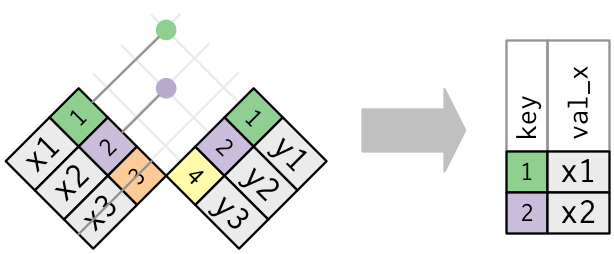
\includegraphics[width=0.4\linewidth]{images/join-semi} \end{center}

\begin{itemize}
\tightlist
\item
  \textbf{\texttt{anti\_join(x,\ y)}} drops all observations in
  \texttt{x} that have a match in \texttt{y}.
\end{itemize}

\begin{center}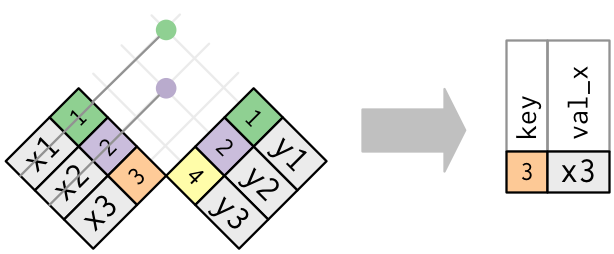
\includegraphics[width=0.4\linewidth]{images/join-anti} \end{center}

\end{frame}

\begin{frame}[fragile]{Filtering joins}

\begin{table}[t]

\caption{\label{tab:unnamed-chunk-53}Patients files}
\centering
\begin{tabular}{l|l|r|l|l}
\hline
First\_Name & Last\_Name & age & sex & adress\\
\hline
John & Smith & 46 & M & 221B Baker Street\\
\hline
Jane & Doe & 33 & F & 57 Rue de Varenne\\
\hline
\end{tabular}
\end{table}

\begin{Shaded}
\begin{Highlighting}[]
\NormalTok{treatments.}\DecValTok{3} \OperatorTok
\StringTok{    }\KeywordTok{separate}\NormalTok{(person,}\DataTypeTok{into =} \KeywordTok{c}\NormalTok{(}\StringTok{"First_Name"}\NormalTok{,}\StringTok{"Last_Name"}\NormalTok{),}\DataTypeTok{sep=}\StringTok{" "}\NormalTok{) }\OperatorTok
\StringTok{    }\KeywordTok{semi_join}\NormalTok{(treatment.meta,}\DataTypeTok{by =} \KeywordTok{c}\NormalTok{(}\StringTok{"First_Name"}\NormalTok{,}\StringTok{"Last_Name"}\NormalTok{))}
\end{Highlighting}
\end{Shaded}

\begin{verbatim}
##   First_Name Last_Name   treatment result
## 1       John     Smith treatment_a     13
## 2       Jane       Doe treatment_a     11
## 3       John     Smith treatment_b     20
## 4       Jane       Doe treatment_b     16
## 5       John     Smith treatment_c     21
## 6       Jane       Doe treatment_c     16
\end{verbatim}

\end{frame}

\begin{frame}[fragile]{Use multiple command together}

\begin{Shaded}
\begin{Highlighting}[]
\NormalTok{iris.tbl}
\end{Highlighting}
\end{Shaded}

\begin{verbatim}
## # A tibble: 150 x 5
##    Sepal.Length Sepal.Width Petal.Length Petal.Width Species
##           <dbl>       <dbl>        <dbl>       <dbl> <fct>  
##  1          5.1         3.5          1.4         0.2 setosa 
##  2          4.9         3            1.4         0.2 setosa 
##  3          4.7         3.2          1.3         0.2 setosa 
##  4          4.6         3.1          1.5         0.2 setosa 
##  5          5           3.6          1.4         0.2 setosa 
##  6          5.4         3.9          1.7         0.4 setosa 
##  7          4.6         3.4          1.4         0.3 setosa 
##  8          5           3.4          1.5         0.2 setosa 
##  9          4.4         2.9          1.4         0.2 setosa 
## 10          4.9         3.1          1.5         0.1 setosa 
## # ... with 140 more rows
\end{verbatim}

\end{frame}

\begin{frame}[fragile]{Use multiple command together}

\begin{Shaded}
\begin{Highlighting}[]
\NormalTok{iris.tbl }\OperatorTok
\StringTok{    }\KeywordTok{gather}\NormalTok{(}\DataTypeTok{key =} \StringTok{"Type"}\NormalTok{,}\DataTypeTok{value =} \StringTok{"obs"}\NormalTok{,}\OperatorTok{-}\NormalTok{Species) }\OperatorTok
\StringTok{    }\KeywordTok{separate}\NormalTok{(Type,}\DataTypeTok{into =} \KeywordTok{c}\NormalTok{(}\StringTok{"Type_1"}\NormalTok{,}\StringTok{"Type_2"}\NormalTok{),}\DataTypeTok{se=}\StringTok{"}\CharTok{\textbackslash{}\textbackslash{}}\StringTok{."}\NormalTok{)}
\end{Highlighting}
\end{Shaded}

\begin{verbatim}
## # A tibble: 600 x 4
##    Species Type_1 Type_2   obs
##    <fct>   <chr>  <chr>  <dbl>
##  1 setosa  Sepal  Length   5.1
##  2 setosa  Sepal  Length   4.9
##  3 setosa  Sepal  Length   4.7
##  4 setosa  Sepal  Length   4.6
##  5 setosa  Sepal  Length   5  
##  6 setosa  Sepal  Length   5.4
##  7 setosa  Sepal  Length   4.6
##  8 setosa  Sepal  Length   5  
##  9 setosa  Sepal  Length   4.4
## 10 setosa  Sepal  Length   4.9
## # ... with 590 more rows
\end{verbatim}

\end{frame}

\begin{frame}[fragile]{Use multiple command together}

\begin{Shaded}
\begin{Highlighting}[]
\NormalTok{iris.tbl }\OperatorTok
\StringTok{    }\KeywordTok{gather}\NormalTok{(}\DataTypeTok{key =} \StringTok{"Type"}\NormalTok{,}\DataTypeTok{value =} \StringTok{"obs"}\NormalTok{,}\OperatorTok{-}\NormalTok{Species) }\OperatorTok
\StringTok{    }\KeywordTok{separate}\NormalTok{(Type,}\DataTypeTok{into =} \KeywordTok{c}\NormalTok{(}\StringTok{"Type_1"}\NormalTok{,}\StringTok{"Type_2"}\NormalTok{),}\DataTypeTok{se=}\StringTok{"}\CharTok{\textbackslash{}\textbackslash{}}\StringTok{."}\NormalTok{) }\OperatorTok
\StringTok{    }\KeywordTok{group_by}\NormalTok{(Species,Type_}\DecValTok{1}\NormalTok{,Type_}\DecValTok{2}\NormalTok{) }\OperatorTok
\StringTok{    }\KeywordTok{mutate}\NormalTok{(}\DataTypeTok{med =} \KeywordTok{median}\NormalTok{(obs))}
\end{Highlighting}
\end{Shaded}

\begin{verbatim}
## # A tibble: 600 x 5
## # Groups:   Species, Type_1, Type_2 [12]
##    Species Type_1 Type_2   obs   med
##    <fct>   <chr>  <chr>  <dbl> <dbl>
##  1 setosa  Sepal  Length   5.1     5
##  2 setosa  Sepal  Length   4.9     5
##  3 setosa  Sepal  Length   4.7     5
##  4 setosa  Sepal  Length   4.6     5
##  5 setosa  Sepal  Length   5       5
##  6 setosa  Sepal  Length   5.4     5
##  7 setosa  Sepal  Length   4.6     5
##  8 setosa  Sepal  Length   5       5
##  9 setosa  Sepal  Length   4.4     5
## 10 setosa  Sepal  Length   4.9     5
## # ... with 590 more rows
\end{verbatim}

\end{frame}

\begin{frame}[fragile]{Use multiple command together}

\small

\begin{Shaded}
\begin{Highlighting}[]
\NormalTok{iris.tbl }\OperatorTok
\StringTok{    }\KeywordTok{gather}\NormalTok{(}\DataTypeTok{key =} \StringTok{"Type"}\NormalTok{,}\DataTypeTok{value =} \StringTok{"obs"}\NormalTok{,}\OperatorTok{-}\NormalTok{Species) }\OperatorTok
\StringTok{    }\KeywordTok{separate}\NormalTok{(Type,}\DataTypeTok{into =} \KeywordTok{c}\NormalTok{(}\StringTok{"Type_1"}\NormalTok{,}\StringTok{"Type_2"}\NormalTok{),}\DataTypeTok{se=}\StringTok{"}\CharTok{\textbackslash{}\textbackslash{}}\StringTok{."}\NormalTok{) }\OperatorTok
\StringTok{    }\KeywordTok{group_by}\NormalTok{(Species,Type_}\DecValTok{1}\NormalTok{,Type_}\DecValTok{2}\NormalTok{) }\OperatorTok
\StringTok{    }\KeywordTok{mutate}\NormalTok{(}\DataTypeTok{med =} \KeywordTok{median}\NormalTok{(obs)) }\OperatorTok
\StringTok{    }\KeywordTok{mutate}\NormalTok{(}\DataTypeTok{Size =} \KeywordTok{ifelse}\NormalTok{(obs }\OperatorTok{<}\StringTok{ }\NormalTok{med,}\StringTok{"Small"}\NormalTok{,}\StringTok{"Big"}\NormalTok{)) }\OperatorTok
\StringTok{    }\KeywordTok{left_join}\NormalTok{(iris.meta,}\DataTypeTok{by =} \StringTok{"Species"}\NormalTok{)}
\end{Highlighting}
\end{Shaded}

\begin{verbatim}
## # A tibble: 600 x 9
## # Groups:   Species, Type_1, Type_2 [?]
##    Species Type_1 Type_2   obs   med Size  Colony Ploidy  `Common name` 
##    <fct>   <chr>  <chr>  <dbl> <dbl> <chr> <chr>  <chr>   <chr>         
##  1 setosa  Sepal  Length   5.1     5 Big   A      diploid Beachhead iris
##  2 setosa  Sepal  Length   4.9     5 Small A      diploid Beachhead iris
##  3 setosa  Sepal  Length   4.7     5 Small A      diploid Beachhead iris
##  4 setosa  Sepal  Length   4.6     5 Small A      diploid Beachhead iris
##  5 setosa  Sepal  Length   5       5 Big   A      diploid Beachhead iris
##  6 setosa  Sepal  Length   5.4     5 Big   A      diploid Beachhead iris
##  7 setosa  Sepal  Length   4.6     5 Small A      diploid Beachhead iris
##  8 setosa  Sepal  Length   5       5 Big   A      diploid Beachhead iris
##  9 setosa  Sepal  Length   4.4     5 Small A      diploid Beachhead iris
## 10 setosa  Sepal  Length   4.9     5 Small A      diploid Beachhead iris
## # ... with 590 more rows
\end{verbatim}

\end{frame}

\begin{frame}[fragile]{Use multiple command together}

\small

\begin{Shaded}
\begin{Highlighting}[]
\NormalTok{iris.tbl }\OperatorTok
\StringTok{    }\KeywordTok{gather}\NormalTok{(}\DataTypeTok{key =} \StringTok{"Type"}\NormalTok{,}\DataTypeTok{value =} \StringTok{"obs"}\NormalTok{,}\OperatorTok{-}\NormalTok{Species) }\OperatorTok
\StringTok{    }\KeywordTok{separate}\NormalTok{(Type,}\DataTypeTok{into =} \KeywordTok{c}\NormalTok{(}\StringTok{"Type_1"}\NormalTok{,}\StringTok{"Type_2"}\NormalTok{),}\DataTypeTok{se=}\StringTok{"}\CharTok{\textbackslash{}\textbackslash{}}\StringTok{."}\NormalTok{) }\OperatorTok
\StringTok{    }\KeywordTok{group_by}\NormalTok{(Species,Type_}\DecValTok{1}\NormalTok{,Type_}\DecValTok{2}\NormalTok{) }\OperatorTok
\StringTok{    }\KeywordTok{mutate}\NormalTok{(}\DataTypeTok{med =} \KeywordTok{median}\NormalTok{(obs)) }\OperatorTok
\StringTok{    }\KeywordTok{mutate}\NormalTok{(}\DataTypeTok{Size =} \KeywordTok{ifelse}\NormalTok{(obs }\OperatorTok{<}\StringTok{ }\NormalTok{med,}\StringTok{"Small"}\NormalTok{,}\StringTok{"Big"}\NormalTok{)) }\OperatorTok
\StringTok{    }\KeywordTok{left_join}\NormalTok{(iris.meta,}\DataTypeTok{by =} \StringTok{"Species"}\NormalTok{) }\OperatorTok
\StringTok{    }\KeywordTok{arrange}\NormalTok{(}\KeywordTok{desc}\NormalTok{(obs)) }\OperatorTok\StringTok{ }\KeywordTok{slice}\NormalTok{(}\DecValTok{1}\NormalTok{)}
\end{Highlighting}
\end{Shaded}

\begin{verbatim}
## # A tibble: 12 x 9
## # Groups:   Species, Type_1, Type_2 [12]
##    Species   Type_1 Type_2   obs   med Size  Colony Ploidy  `Common name`  
##    <fct>     <chr>  <chr>  <dbl> <dbl> <chr> <chr>  <chr>   <chr>          
##  1 setosa    Petal  Length   1.9  1.5  Big   A      diploid Beachhead iris 
##  2 setosa    Petal  Width    0.6  0.2  Big   A      diploid Beachhead iris 
##  3 setosa    Sepal  Length   5.8  5    Big   A      diploid Beachhead iris 
##  4 setosa    Sepal  Width    4.4  3.4  Big   A      diploid Beachhead iris 
##  5 versicol~ Petal  Length   5.1  4.35 Big   A      hexapl~ Harlequin blue~
##  6 versicol~ Petal  Width    1.8  1.3  Big   A      hexapl~ Harlequin blue~
##  7 versicol~ Sepal  Length   7    5.9  Big   A      hexapl~ Harlequin blue~
##  8 versicol~ Sepal  Width    3.4  2.8  Big   A      hexapl~ Harlequin blue~
##  9 virginica Petal  Length   6.9  5.55 Big   B      tetrap~ Virginia iris  
## 10 virginica Petal  Width    2.5  2    Big   B      tetrap~ Virginia iris  
## 11 virginica Sepal  Length   7.9  6.5  Big   B      tetrap~ Virginia iris  
## 12 virginica Sepal  Width    3.8  3    Big   B      tetrap~ Virginia iris
\end{verbatim}

\end{frame}

\section{\texorpdfstring{Data visualisation using
\texttt{ggplot2}}{Data visualisation using ggplot2}}\label{data-visualisation-using-ggplot2}

\begin{frame}[fragile]{A base plot}

\centering

\begin{Shaded}
\begin{Highlighting}[]
\KeywordTok{plot}\NormalTok{(Petal.Width}\OperatorTok{~}\NormalTok{Petal.Length,}\DataTypeTok{data=}\NormalTok{iris.tbl)}
\end{Highlighting}
\end{Shaded}

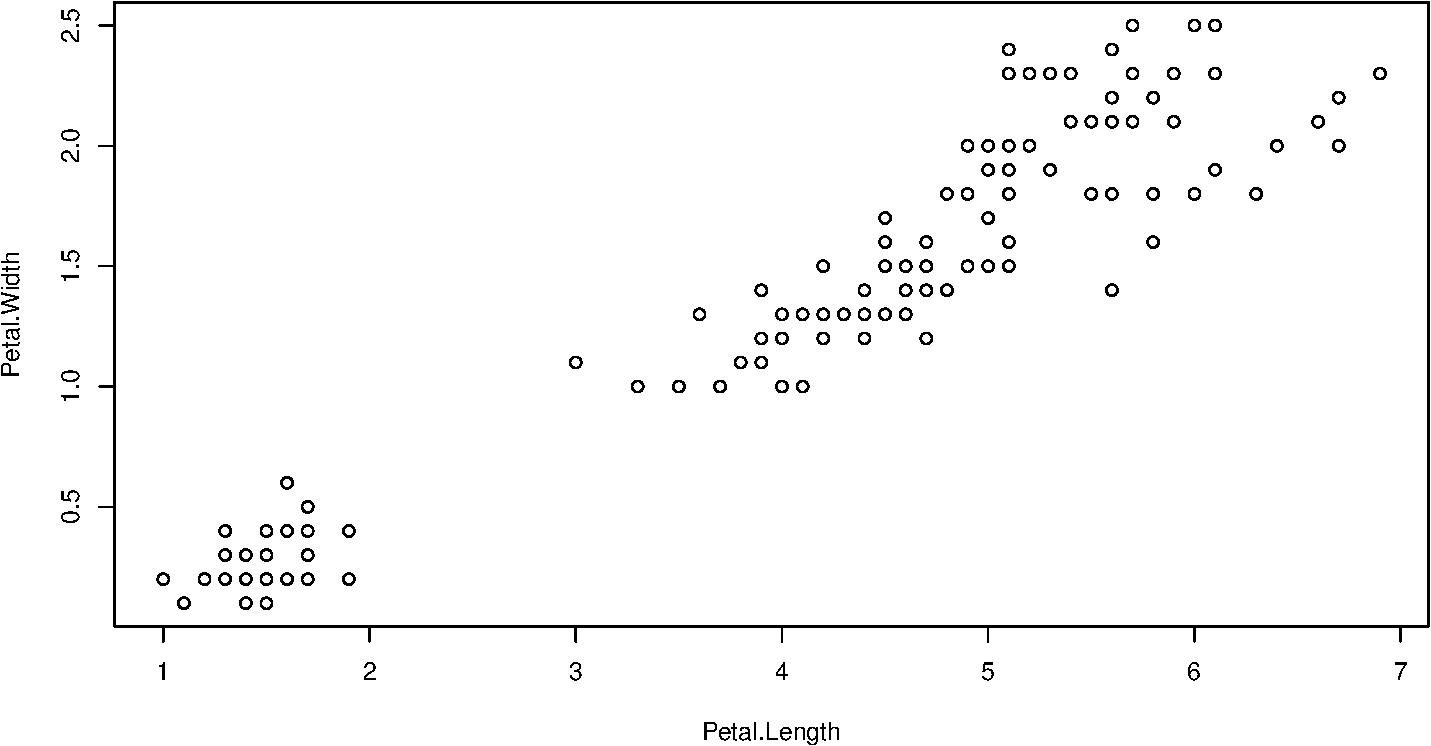
\includegraphics{tidyverse_28_03_files/figure-beamer/base_plot1-1.pdf}

\end{frame}

\begin{frame}[fragile]{A ggplot2 plot}

\centering

\begin{Shaded}
\begin{Highlighting}[]
\NormalTok{iris.tbl }\OperatorTok\StringTok{ }\KeywordTok{ggplot}\NormalTok{(}\KeywordTok{aes}\NormalTok{(}\DataTypeTok{x=}\NormalTok{Petal.Width,}\DataTypeTok{y=}\NormalTok{Petal.Length)) }\OperatorTok{+}
\StringTok{    }\KeywordTok{geom_point}\NormalTok{()}
\end{Highlighting}
\end{Shaded}

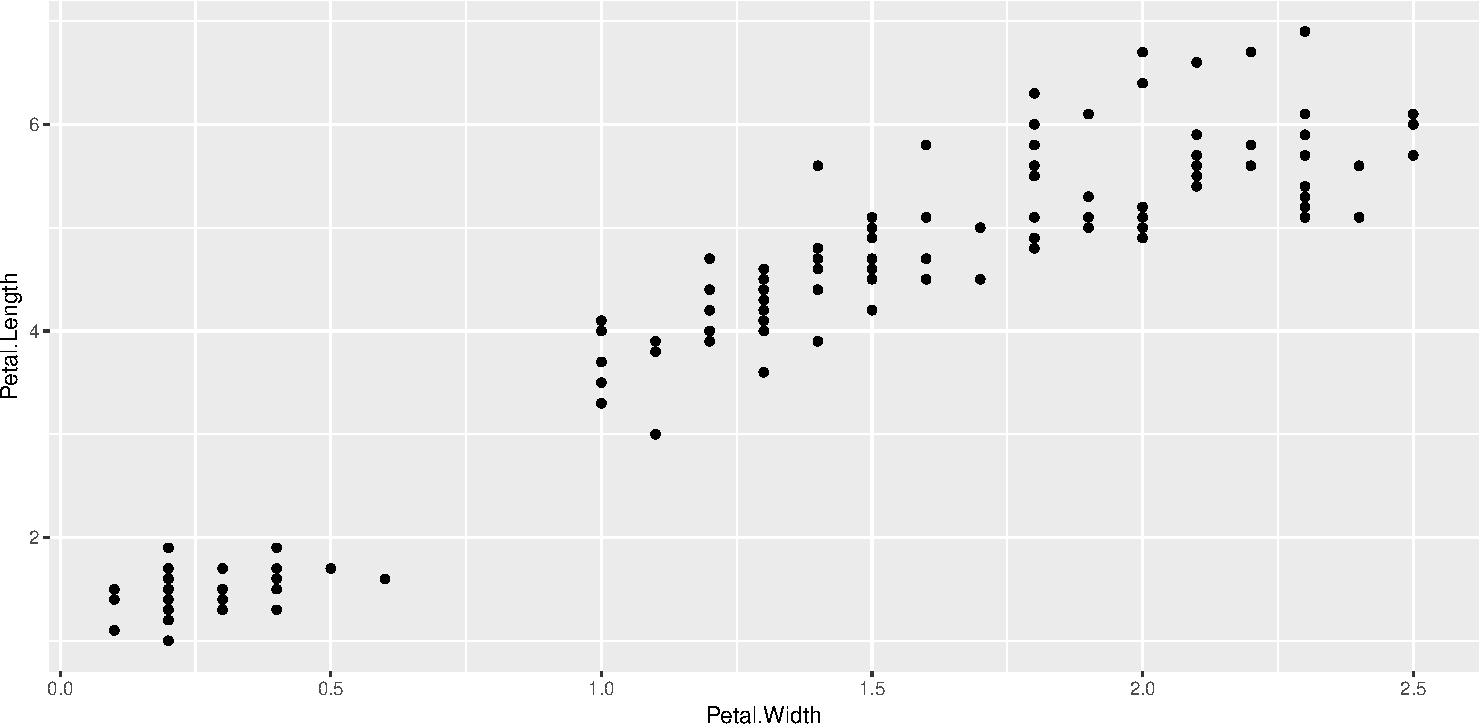
\includegraphics{tidyverse_28_03_files/figure-beamer/ggplot1-1.pdf}

\end{frame}

\begin{frame}[fragile]{A ggplot2 plot}

\centering

\begin{Shaded}
\begin{Highlighting}[]
\NormalTok{iris.tbl }\OperatorTok\StringTok{ }\KeywordTok{ggplot}\NormalTok{(}\KeywordTok{aes}\NormalTok{(}\DataTypeTok{x=}\NormalTok{Petal.Width,}\DataTypeTok{y=}\NormalTok{Petal.Length)) }\OperatorTok{+}
\StringTok{    }\KeywordTok{geom_point}\NormalTok{() }\OperatorTok{+}
\StringTok{    }\KeywordTok{geom_smooth}\NormalTok{(}\DataTypeTok{method =} \StringTok{"lm"}\NormalTok{)}
\end{Highlighting}
\end{Shaded}

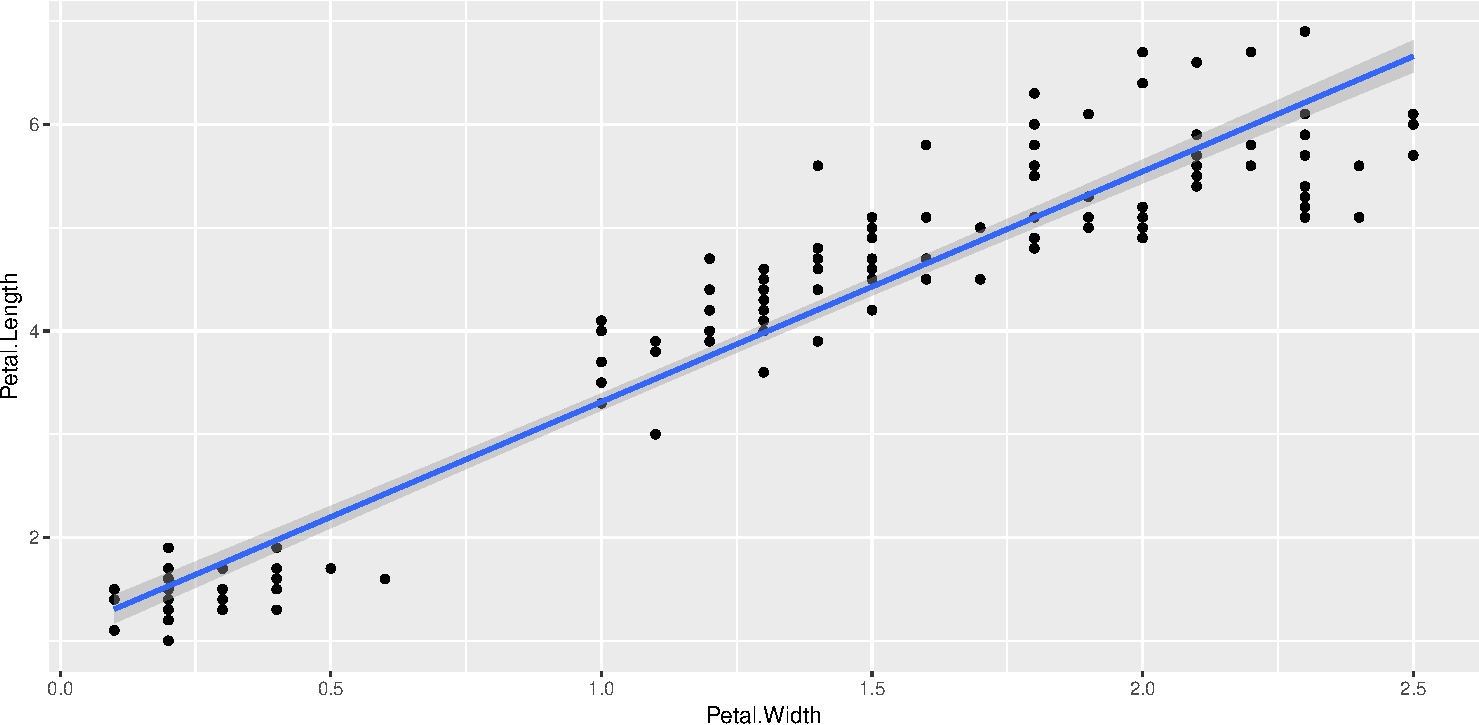
\includegraphics{tidyverse_28_03_files/figure-beamer/ggplot2-1.pdf}

\end{frame}

\begin{frame}{The three key components of every ggplot2}

\Large

The three components of every graphics :

\begin{itemize}
\tightlist
\item
  \textbf{data}: the dataset who's need to be plotted.
\item
  \textbf{aesthetics}: aesthetics mapping between variables in the data
  (x,y,visuals properties, \ldots{}).
\item
  \textbf{geoms}: one or more layers to render each observations.
\end{itemize}

\begin{center}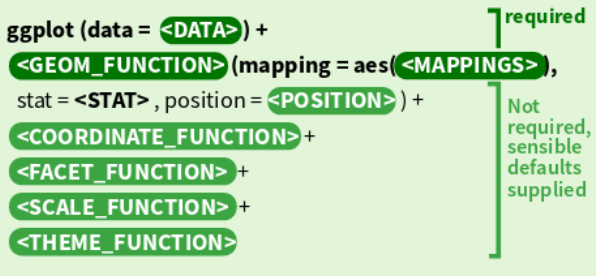
\includegraphics[width=0.8\linewidth]{images/3ggplot2} \end{center}

\end{frame}

\begin{frame}[fragile]{The three key components of every ggplot2}

\Large

The three components of every graphics :

\begin{itemize}
\tightlist
\item
  \textbf{data}: the dataset who's need to be plotted.
\item
  \textbf{aesthetics}: aesthetics mapping between variables in the data
  (x,y,visuals properties, \ldots{}).
\item
  \textbf{geoms}: one or more layers to render each observations.
\end{itemize}

\begin{Shaded}
\begin{Highlighting}[]
\NormalTok{p <-}\StringTok{ }\NormalTok{iris.tbl }\OperatorTok\CommentTok{# Data}
\StringTok{    }\KeywordTok{ggplot}\NormalTok{(}\KeywordTok{aes}\NormalTok{(}\DataTypeTok{x=}\NormalTok{Petal.Width,}\DataTypeTok{y=}\NormalTok{Petal.Length)) }\OperatorTok{+}\CommentTok{# aesthetics}
\StringTok{    }\KeywordTok{geom_point}\NormalTok{()}\CommentTok{# Layer: points}
\end{Highlighting}
\end{Shaded}

Add layer : smooth with linear model

\begin{Shaded}
\begin{Highlighting}[]
\NormalTok{p }\OperatorTok{+}\StringTok{ }\KeywordTok{geom_smooth}\NormalTok{(}\DataTypeTok{method =} \StringTok{"lm"}\NormalTok{)}
\end{Highlighting}
\end{Shaded}

More you add components with \texttt{+}, more you'll build sophisticated
plots.

\end{frame}

\begin{frame}[fragile]{Add more aesthetics}

\begin{Shaded}
\begin{Highlighting}[]
\NormalTok{p <-}\StringTok{ }\NormalTok{iris.tbl }\OperatorTok\CommentTok{# Data}
\StringTok{    }\KeywordTok{ggplot}\NormalTok{(}\KeywordTok{aes}\NormalTok{(}\DataTypeTok{x=}\NormalTok{Petal.Width,}\DataTypeTok{y=}\NormalTok{Petal.Length,}\DataTypeTok{col=}\NormalTok{Species)) }\OperatorTok{+}\CommentTok{# aesthetics}
\StringTok{    }\KeywordTok{geom_point}\NormalTok{()}\CommentTok{# Layer: points}
\KeywordTok{print}\NormalTok{(p)}
\end{Highlighting}
\end{Shaded}

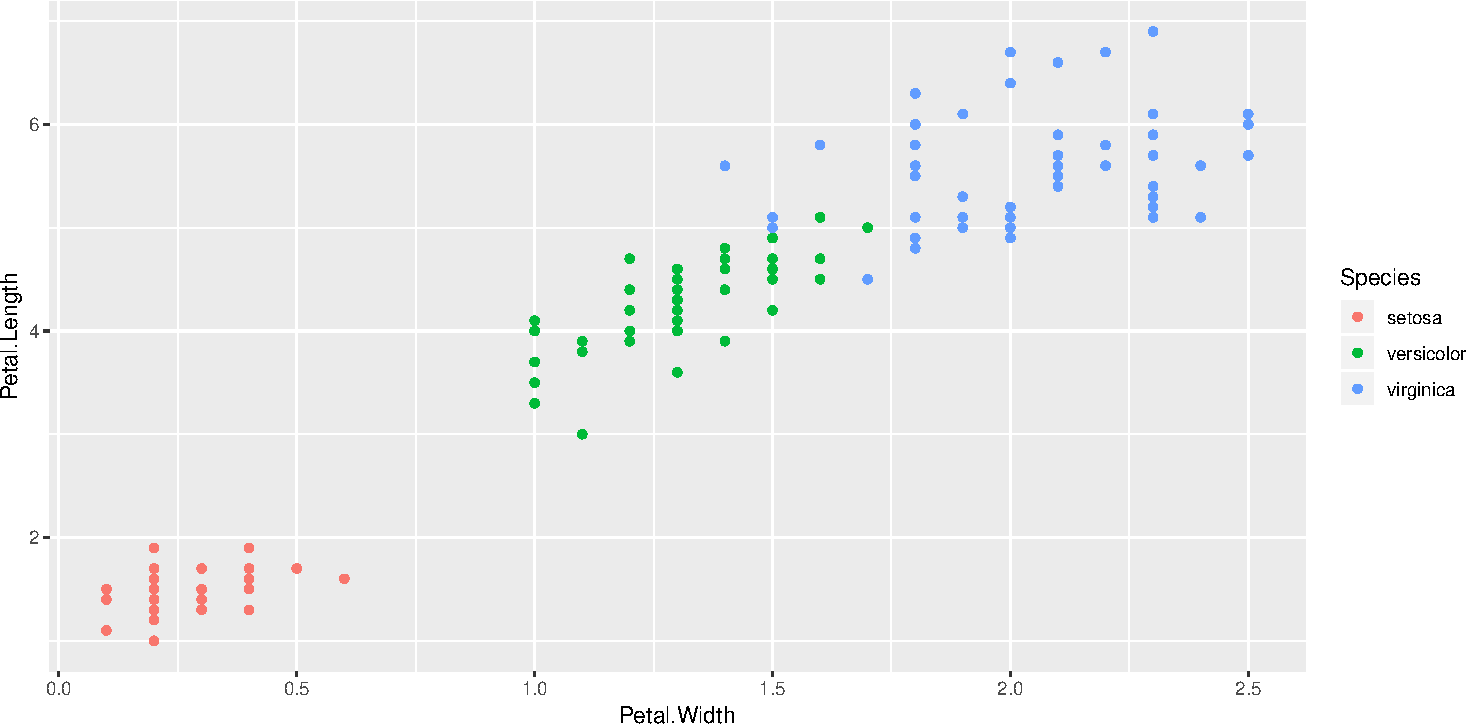
\includegraphics{tidyverse_28_03_files/figure-beamer/ggplot5-1.pdf}

\end{frame}

\begin{frame}[fragile]{Add more aesthetics}

\begin{Shaded}
\begin{Highlighting}[]
\NormalTok{p }\OperatorTok{+}\StringTok{ }\KeywordTok{geom_smooth}\NormalTok{(}\DataTypeTok{method =} \StringTok{"lm"}\NormalTok{)}
\end{Highlighting}
\end{Shaded}

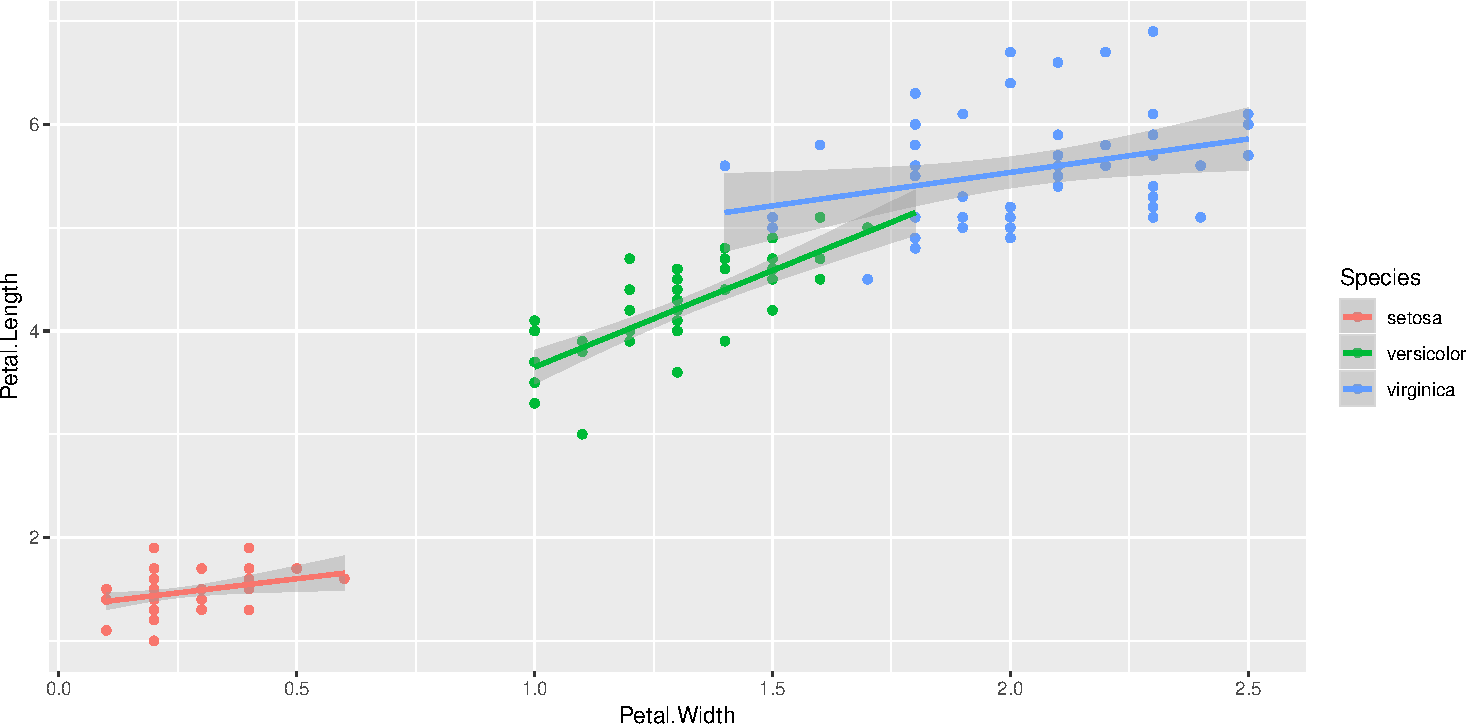
\includegraphics{tidyverse_28_03_files/figure-beamer/ggplot6-1.pdf}

\end{frame}

\begin{frame}[fragile]{Add more aesthetics}

\begin{Shaded}
\begin{Highlighting}[]
\NormalTok{p <-}\StringTok{ }\NormalTok{iris.tbl }\OperatorTok\CommentTok{# Data}
\StringTok{    }\KeywordTok{ggplot}\NormalTok{(}\KeywordTok{aes}\NormalTok{(}\DataTypeTok{x=}\NormalTok{Petal.Width,}\DataTypeTok{y=}\NormalTok{Petal.Length)) }\OperatorTok{+}\CommentTok{# aesthetics}
\StringTok{    }\KeywordTok{geom_point}\NormalTok{(}\KeywordTok{aes}\NormalTok{(}\DataTypeTok{col=}\NormalTok{Species)) }\OperatorTok{+}\CommentTok{# Layer: points}
\StringTok{    }\KeywordTok{geom_smooth}\NormalTok{(}\DataTypeTok{method =} \StringTok{"lm"}\NormalTok{)}
\KeywordTok{print}\NormalTok{(p)}
\end{Highlighting}
\end{Shaded}

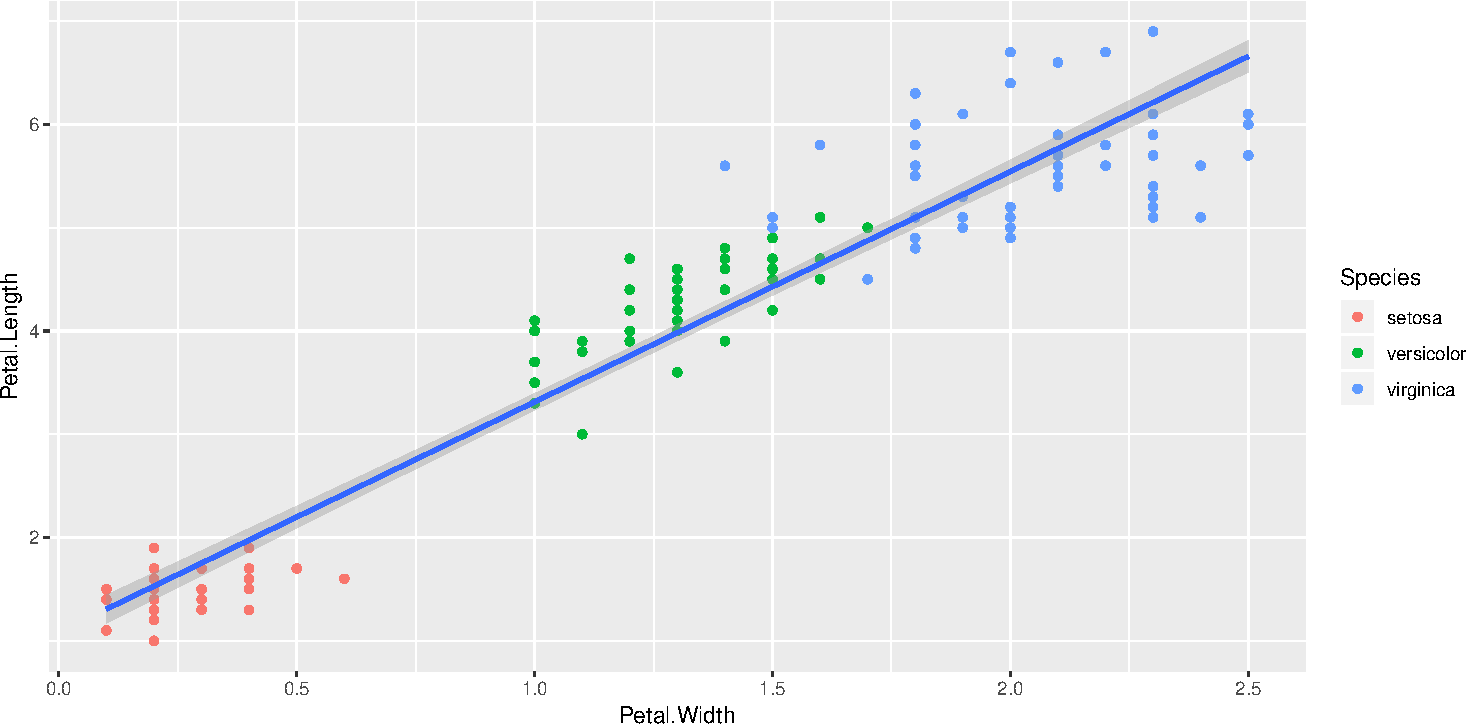
\includegraphics{tidyverse_28_03_files/figure-beamer/ggplot7-1.pdf}

\end{frame}

\begin{frame}[fragile]{Other aesthetics attributes}

\begin{Shaded}
\begin{Highlighting}[]
\NormalTok{p <-}\StringTok{ }\NormalTok{iris.tbl }\OperatorTok\CommentTok{# Data}
\StringTok{    }\KeywordTok{ggplot}\NormalTok{(}\KeywordTok{aes}\NormalTok{(}\DataTypeTok{x=}\NormalTok{Petal.Width,}\DataTypeTok{y=}\NormalTok{Petal.Length)) }\OperatorTok{+}\CommentTok{# aesthetics}
\StringTok{    }\KeywordTok{geom_point}\NormalTok{(}\KeywordTok{aes}\NormalTok{(}\DataTypeTok{shape=}\NormalTok{Species))}\CommentTok{# Layer: points}
\KeywordTok{print}\NormalTok{(p)}
\end{Highlighting}
\end{Shaded}

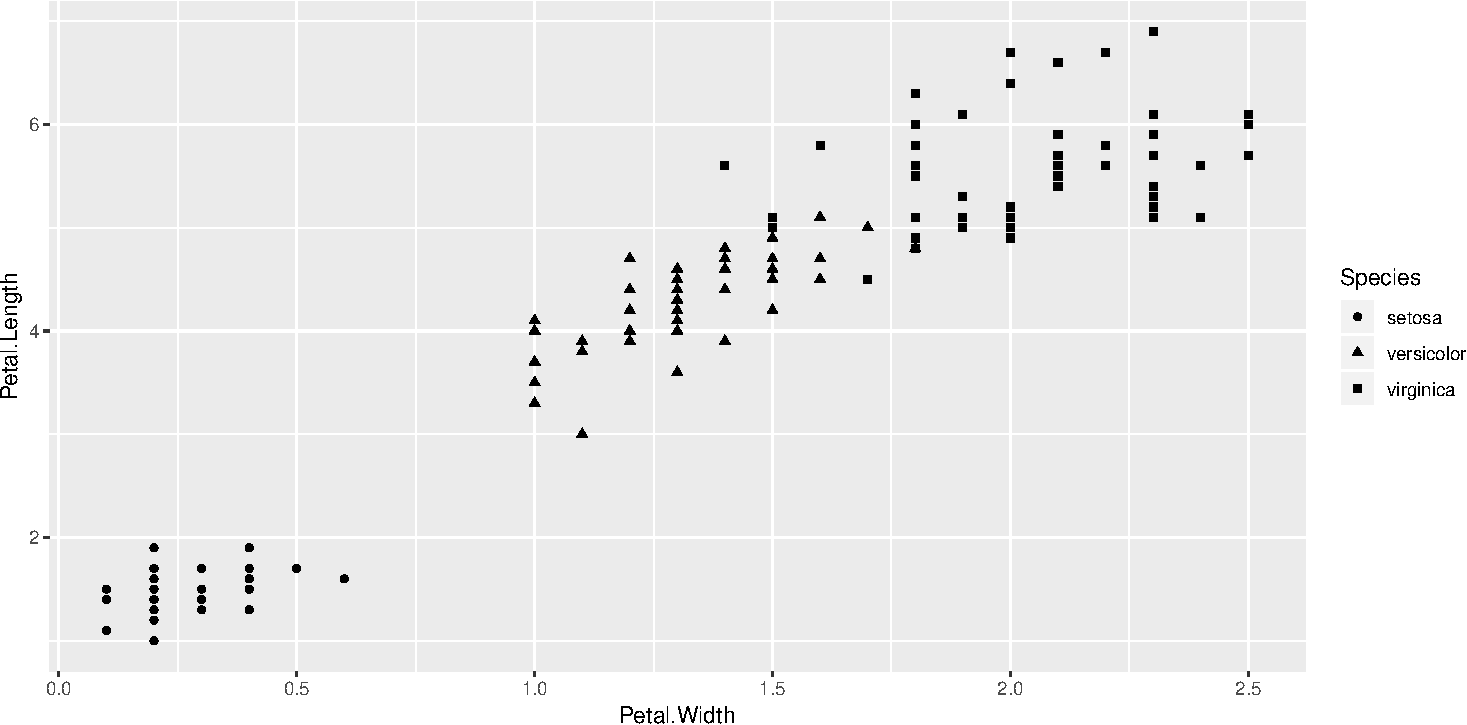
\includegraphics{tidyverse_28_03_files/figure-beamer/ggplot8-1.pdf}

\end{frame}

\begin{frame}[fragile]{Other aesthetics attributes}

\begin{Shaded}
\begin{Highlighting}[]
\NormalTok{p <-}\StringTok{ }\NormalTok{iris.tbl }\OperatorTok\CommentTok{# Data}
\StringTok{    }\KeywordTok{ggplot}\NormalTok{(}\KeywordTok{aes}\NormalTok{(}\DataTypeTok{x=}\NormalTok{Petal.Width,}\DataTypeTok{y=}\NormalTok{Petal.Length)) }\OperatorTok{+}\CommentTok{# aesthetics}
\StringTok{    }\KeywordTok{geom_point}\NormalTok{(}\KeywordTok{aes}\NormalTok{(}\DataTypeTok{col=}\NormalTok{Species,}\DataTypeTok{size =}\NormalTok{ Sepal.Length))}\CommentTok{# Layer: points}
\KeywordTok{print}\NormalTok{(p)}
\end{Highlighting}
\end{Shaded}

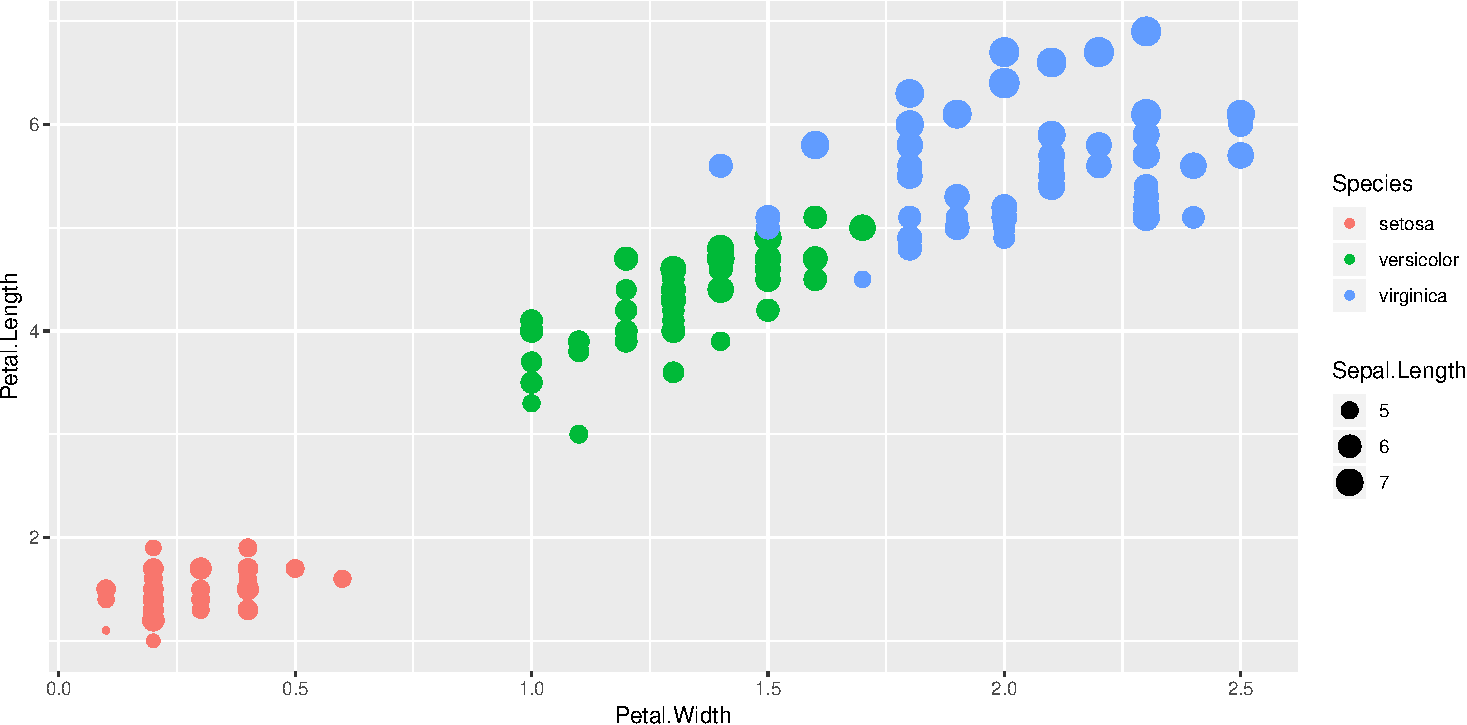
\includegraphics{tidyverse_28_03_files/figure-beamer/ggplot9-1.pdf}

\end{frame}

\begin{frame}[fragile]{Use fixed value}

\begin{Shaded}
\begin{Highlighting}[]
\NormalTok{p <-}\StringTok{ }\NormalTok{iris.tbl }\OperatorTok\CommentTok{# Data}
\StringTok{    }\KeywordTok{ggplot}\NormalTok{(}\KeywordTok{aes}\NormalTok{(}\DataTypeTok{x=}\NormalTok{Petal.Width,}\DataTypeTok{y=}\NormalTok{Petal.Length)) }\OperatorTok{+}\CommentTok{# aesthetics}
\StringTok{    }\KeywordTok{geom_point}\NormalTok{(}\DataTypeTok{col=}\StringTok{"blue"}\NormalTok{,}\DataTypeTok{size=}\DecValTok{4}\NormalTok{) }\OperatorTok{+}\CommentTok{# Layer: points}
\StringTok{    }\KeywordTok{geom_smooth}\NormalTok{(}\DataTypeTok{method =} \StringTok{"lm"}\NormalTok{,}\DataTypeTok{col=}\StringTok{"red"}\NormalTok{,}\DataTypeTok{fill=}\StringTok{"orange"}\NormalTok{)}
\KeywordTok{print}\NormalTok{(p)}
\end{Highlighting}
\end{Shaded}

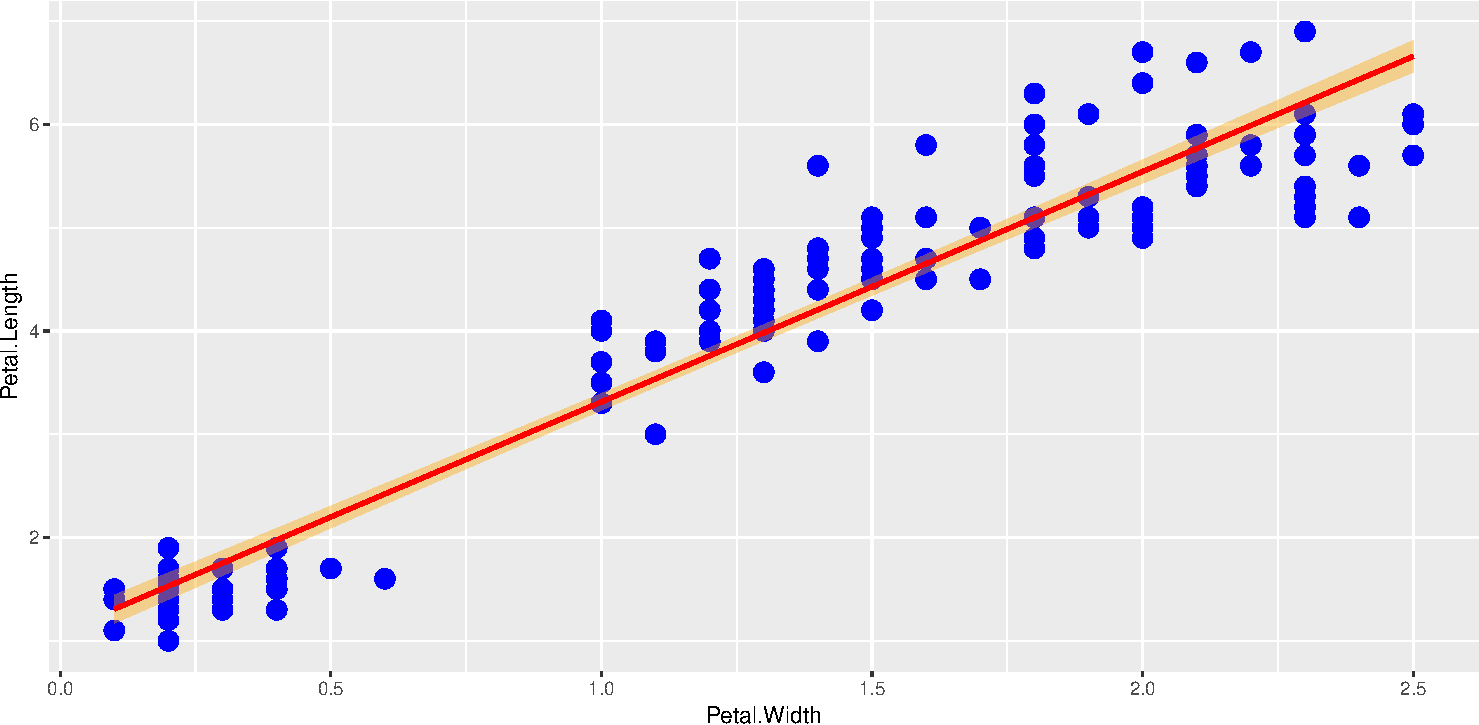
\includegraphics{tidyverse_28_03_files/figure-beamer/ggplot10-1.pdf}

\end{frame}

\begin{frame}{Plot geoms}

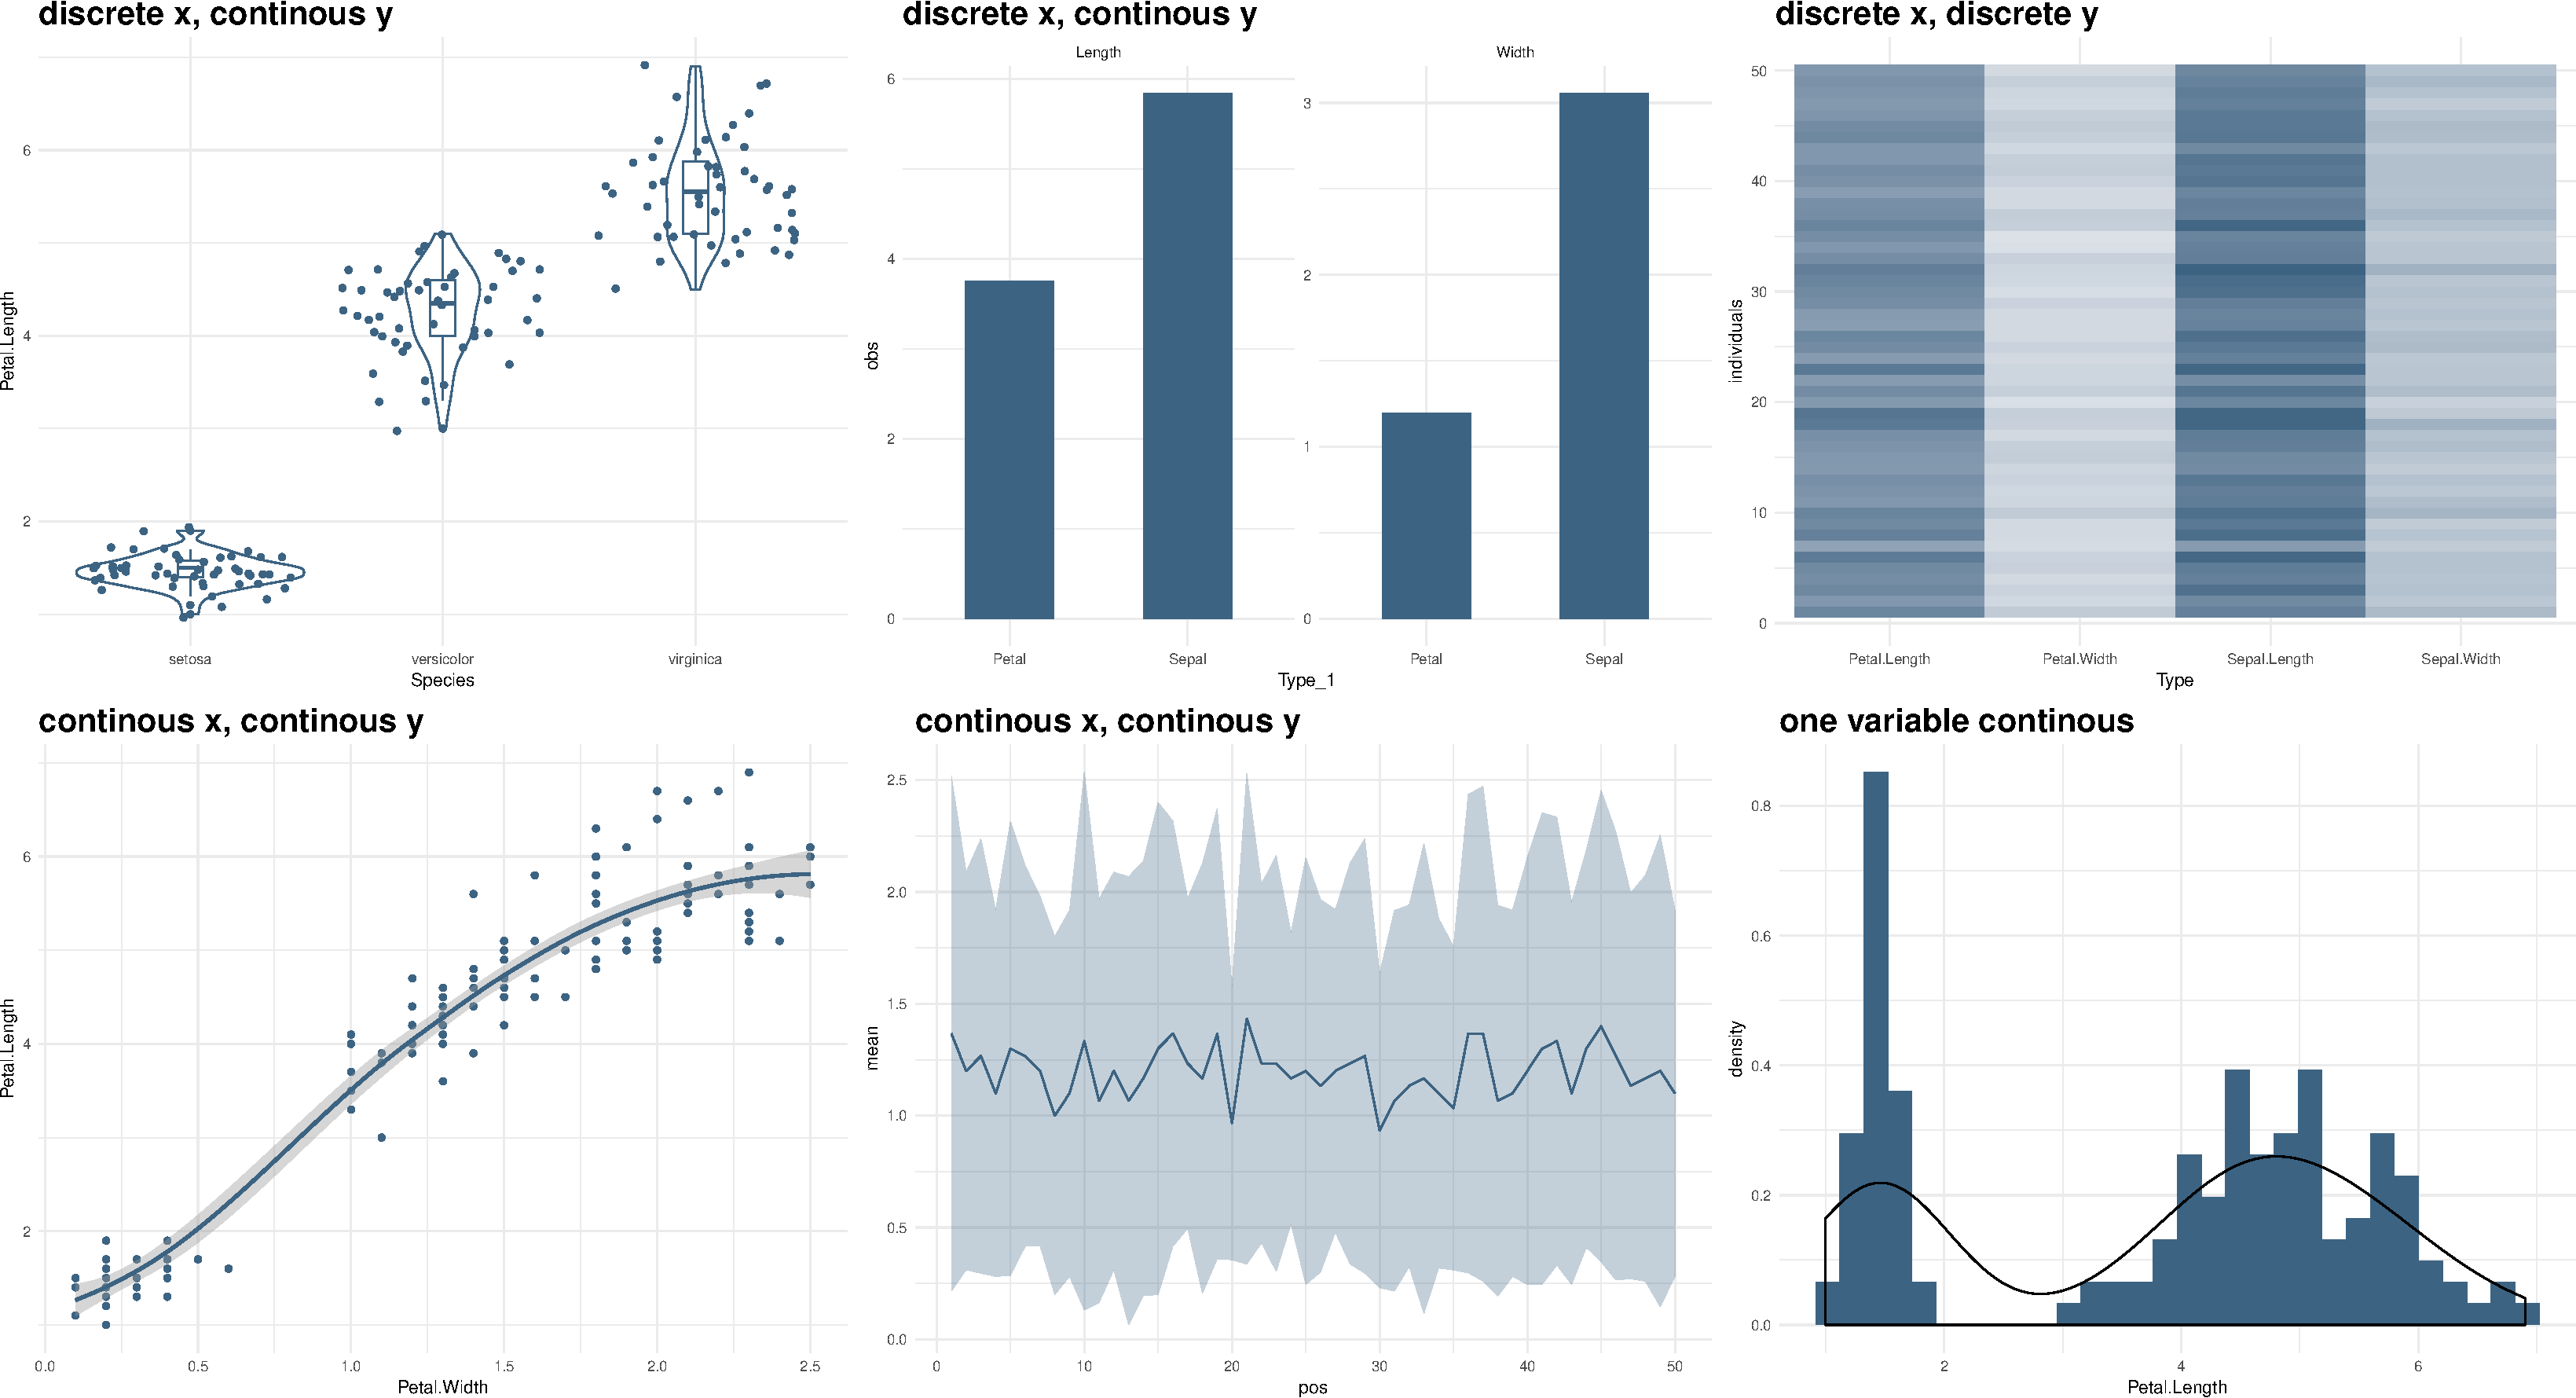
\includegraphics{tidyverse_28_03_files/figure-beamer/ggplot11-1.pdf}

\end{frame}

\begin{frame}[fragile]{Facetting}

\textbf{Facetting}:

\begin{itemize}
\tightlist
\item
  \texttt{facet\_grid(variable\textasciitilde{}foliaces)} : Display all
  possibility even if some plots are \textbf{empty}.
\item
  \texttt{facet\_wrap(variable\textasciitilde{}foliaces)} : Display only
  the plots having actual values.
\end{itemize}

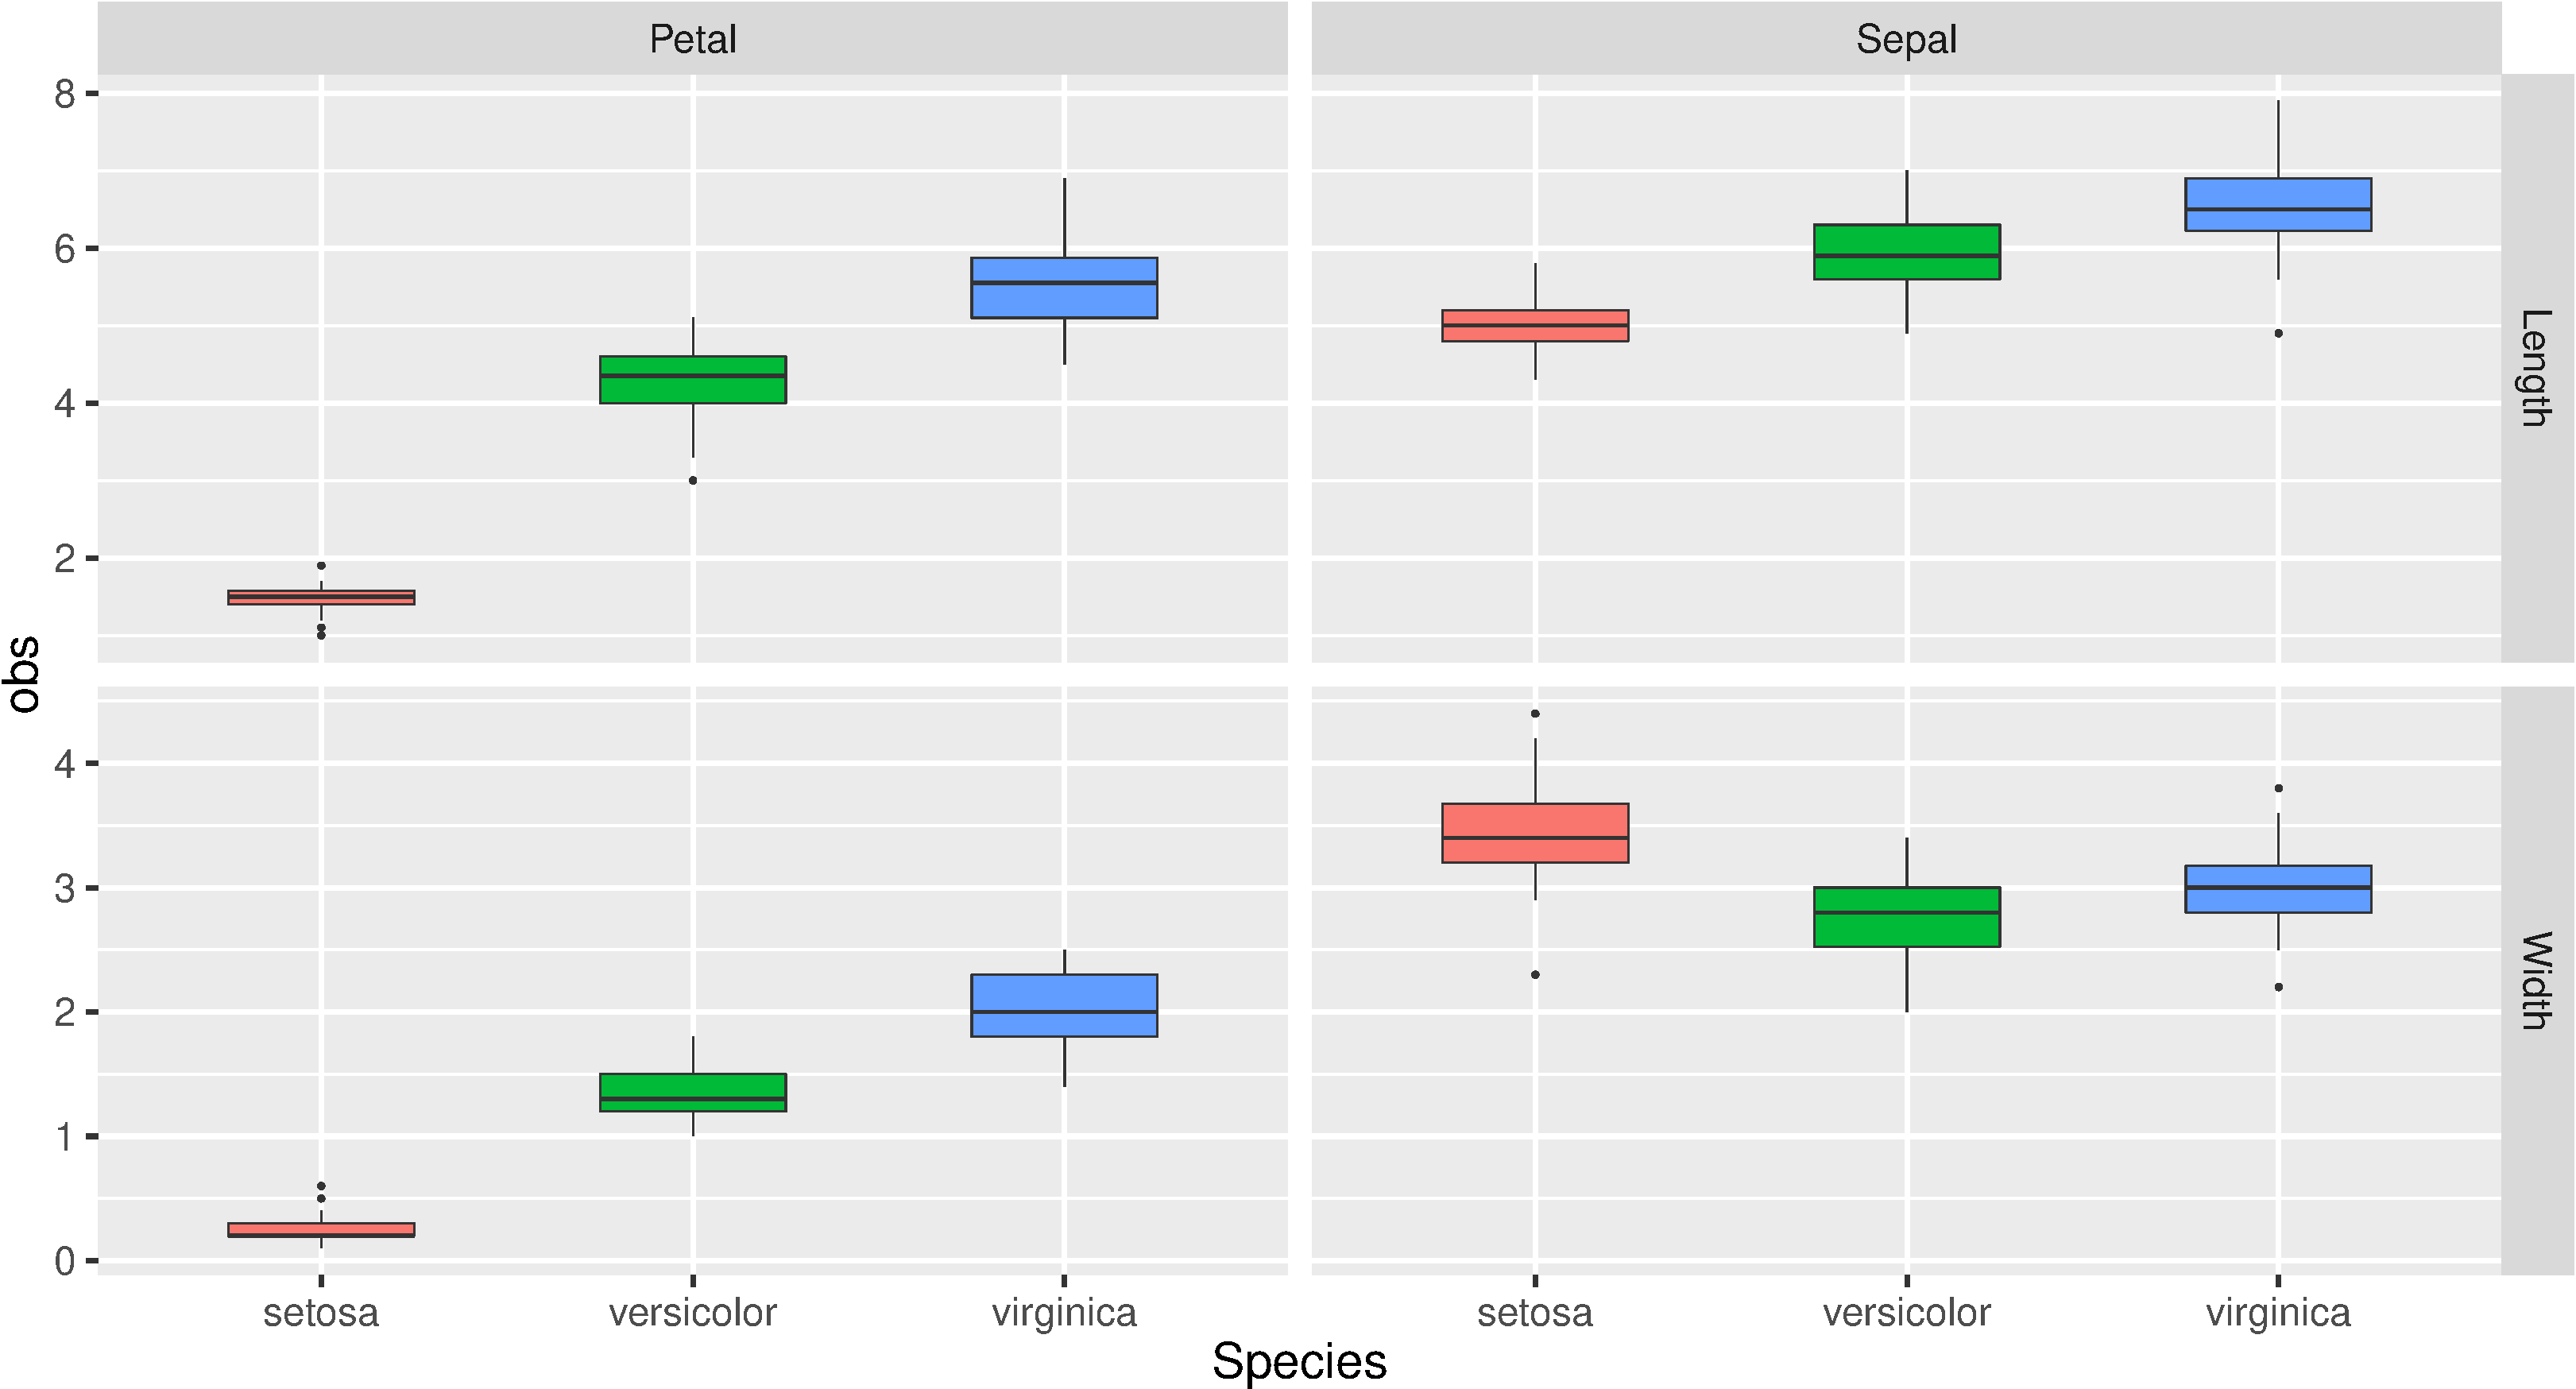
\includegraphics{tidyverse_28_03_files/figure-beamer/ggplot12-1.pdf}

\end{frame}

\begin{frame}[fragile]{Graphical options}

\begin{Shaded}
\begin{Highlighting}[]
\NormalTok{p <-}\StringTok{ }\NormalTok{iris.tbl }\OperatorTok\CommentTok{# Data}
\StringTok{    }\KeywordTok{ggplot}\NormalTok{(}\KeywordTok{aes}\NormalTok{(}\DataTypeTok{x=}\NormalTok{Petal.Width,}\DataTypeTok{y=}\NormalTok{Petal.Length)) }\OperatorTok{+}\CommentTok{# aesthetics}
\StringTok{    }\KeywordTok{geom_point}\NormalTok{(}\KeywordTok{aes}\NormalTok{(}\DataTypeTok{col=}\NormalTok{Species,}\DataTypeTok{size =}\NormalTok{ Sepal.Length)) }\OperatorTok{+}\CommentTok{# Layer: points}
\StringTok{    }\KeywordTok{scale_color_brewer}\NormalTok{(}\DataTypeTok{palette=}\StringTok{"Set3"}\NormalTok{) }\CommentTok{#A new palette}
\KeywordTok{print}\NormalTok{(p)}
\end{Highlighting}
\end{Shaded}

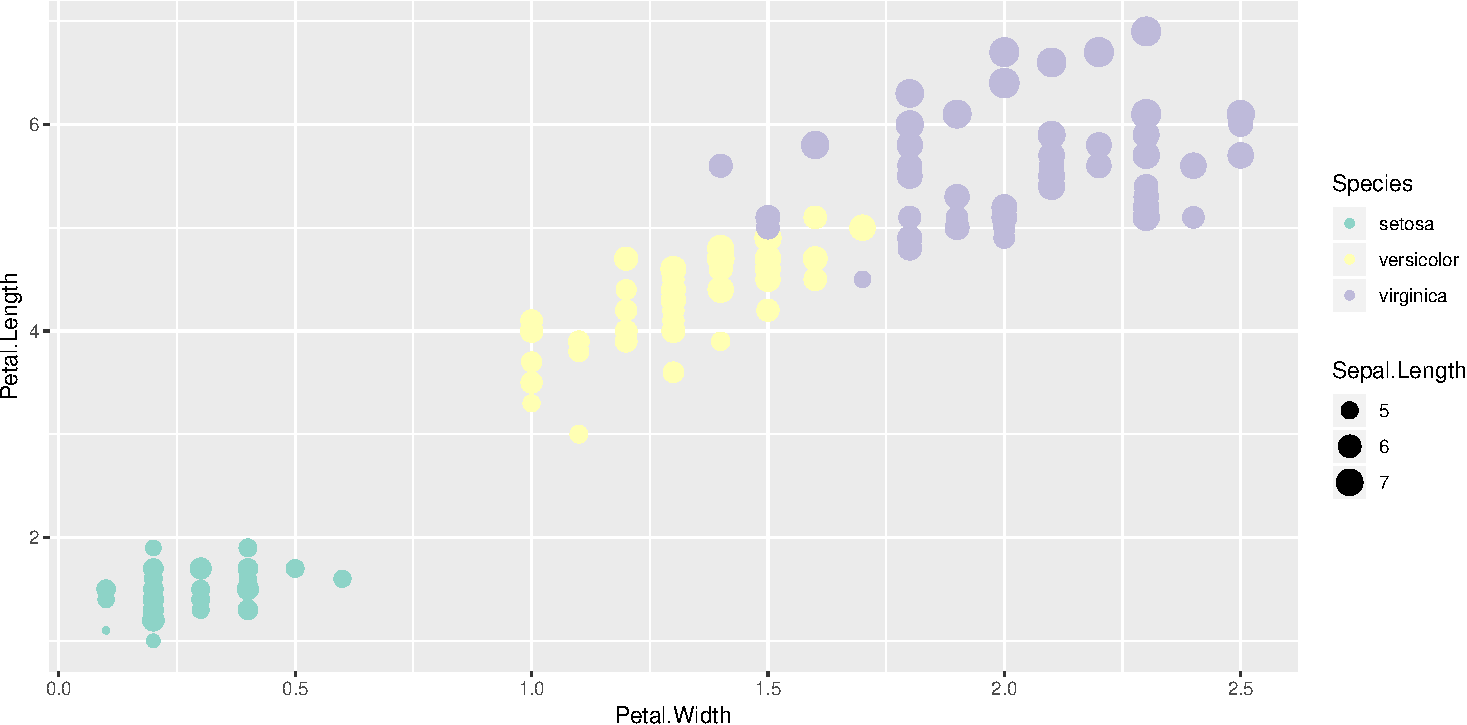
\includegraphics{tidyverse_28_03_files/figure-beamer/ggplot13-1.pdf}

\end{frame}

\begin{frame}[fragile]{Graphical options}

\begin{Shaded}
\begin{Highlighting}[]
\NormalTok{p <-}\StringTok{ }\NormalTok{iris.tbl }\OperatorTok\CommentTok{# Data}
\StringTok{    }\KeywordTok{ggplot}\NormalTok{(}\KeywordTok{aes}\NormalTok{(}\DataTypeTok{x=}\NormalTok{Petal.Width,}\DataTypeTok{y=}\NormalTok{Petal.Length)) }\OperatorTok{+}\CommentTok{# aesthetics}
\StringTok{    }\KeywordTok{geom_point}\NormalTok{(}\KeywordTok{aes}\NormalTok{(}\DataTypeTok{col=}\NormalTok{Species,}\DataTypeTok{size =}\NormalTok{ Sepal.Length)) }\OperatorTok{+}\CommentTok{# Layer: points}
\StringTok{    }\KeywordTok{scale_color_manual}\NormalTok{(}\DataTypeTok{values =} \KeywordTok{c}\NormalTok{(}\StringTok{"red"}\NormalTok{,}\StringTok{"blue"}\NormalTok{,}\StringTok{"green"}\NormalTok{),  }\CommentTok{#A new palette}
                       \DataTypeTok{labels =} \KeywordTok{c}\NormalTok{(}\StringTok{"Setosa"}\NormalTok{,}\StringTok{"Versicolor"}\NormalTok{,}\StringTok{"Virginica"}\NormalTok{))}
\KeywordTok{print}\NormalTok{(p)}
\end{Highlighting}
\end{Shaded}

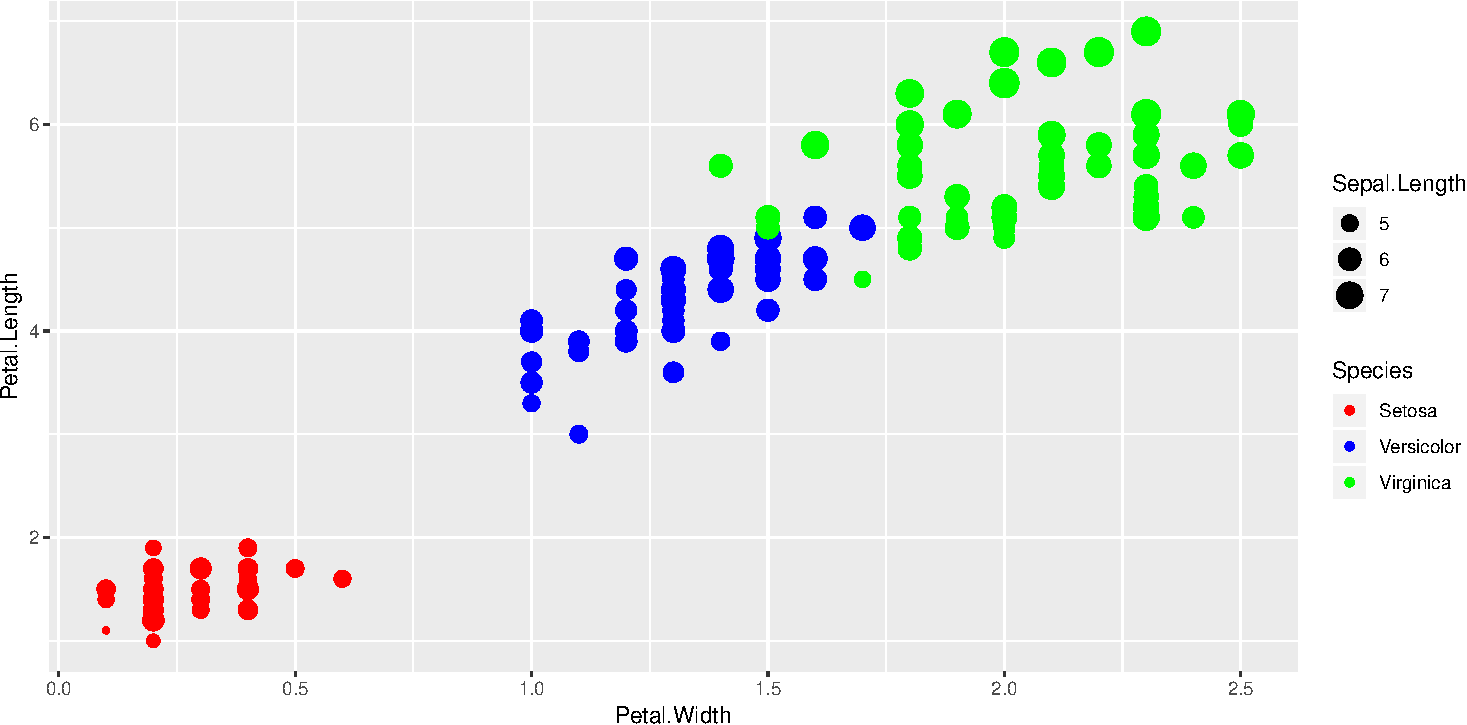
\includegraphics{tidyverse_28_03_files/figure-beamer/ggplot14-1.pdf}

\end{frame}

\begin{frame}{Themes}

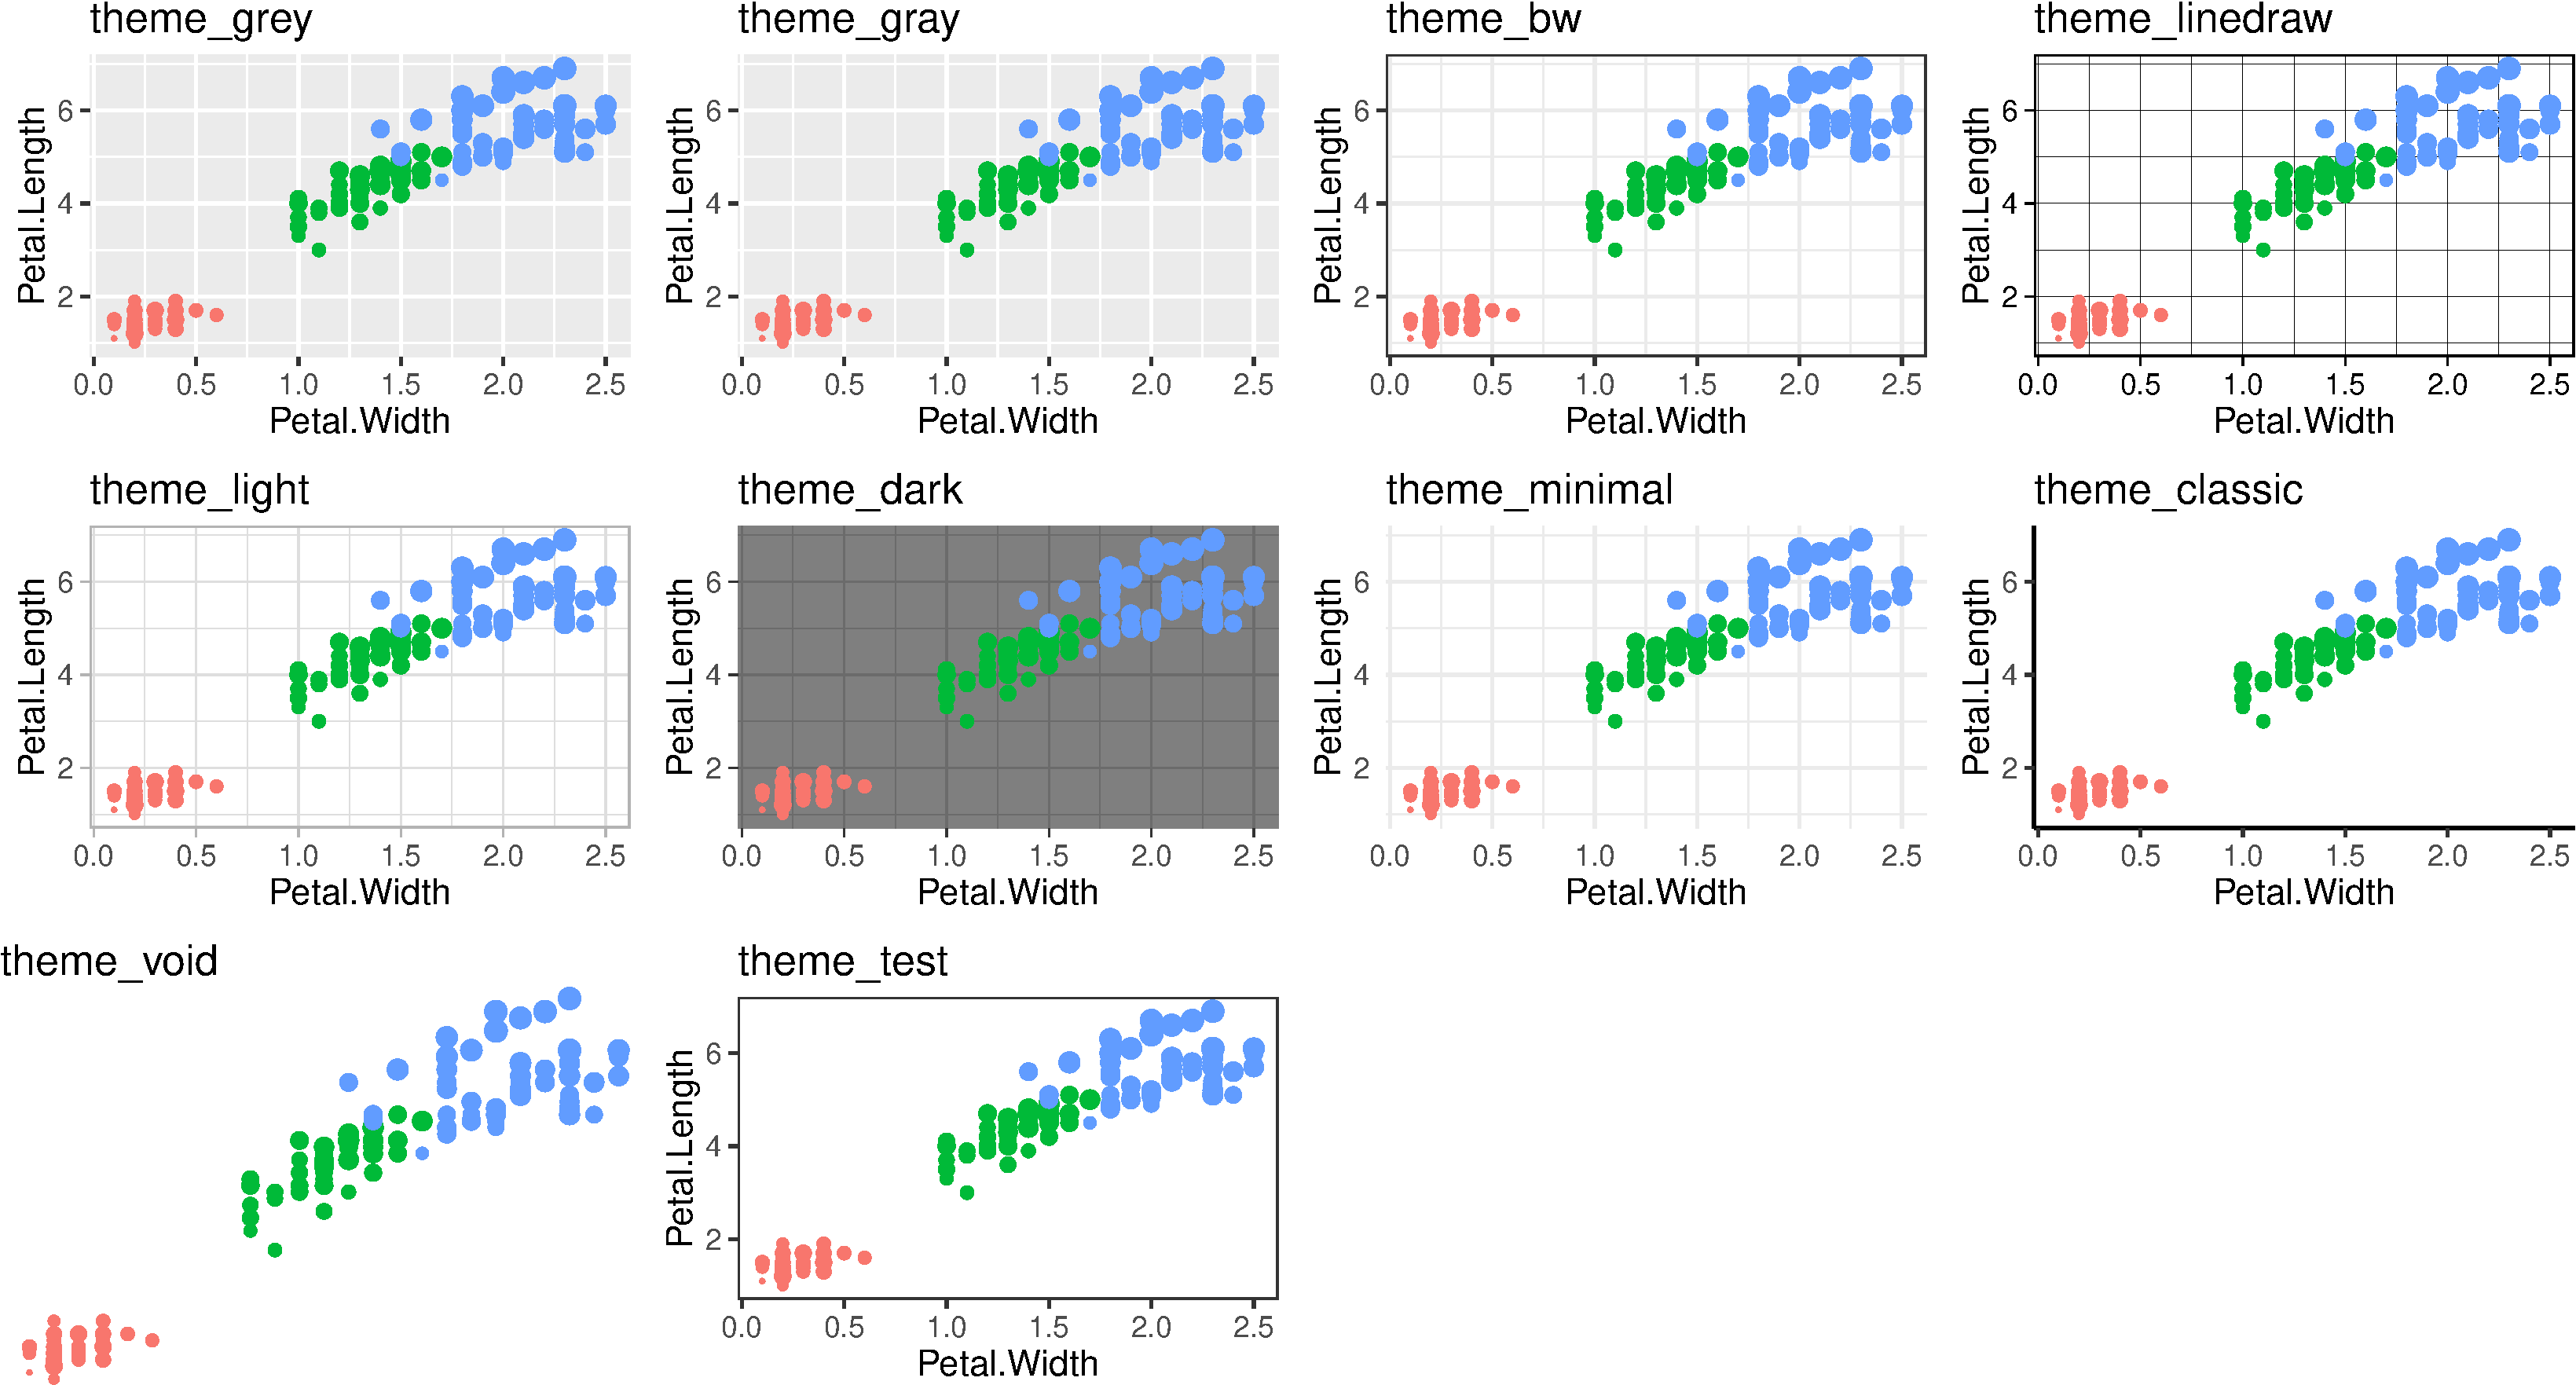
\includegraphics{tidyverse_28_03_files/figure-beamer/ggplot15-1.pdf}

\end{frame}

\begin{frame}{Themes}

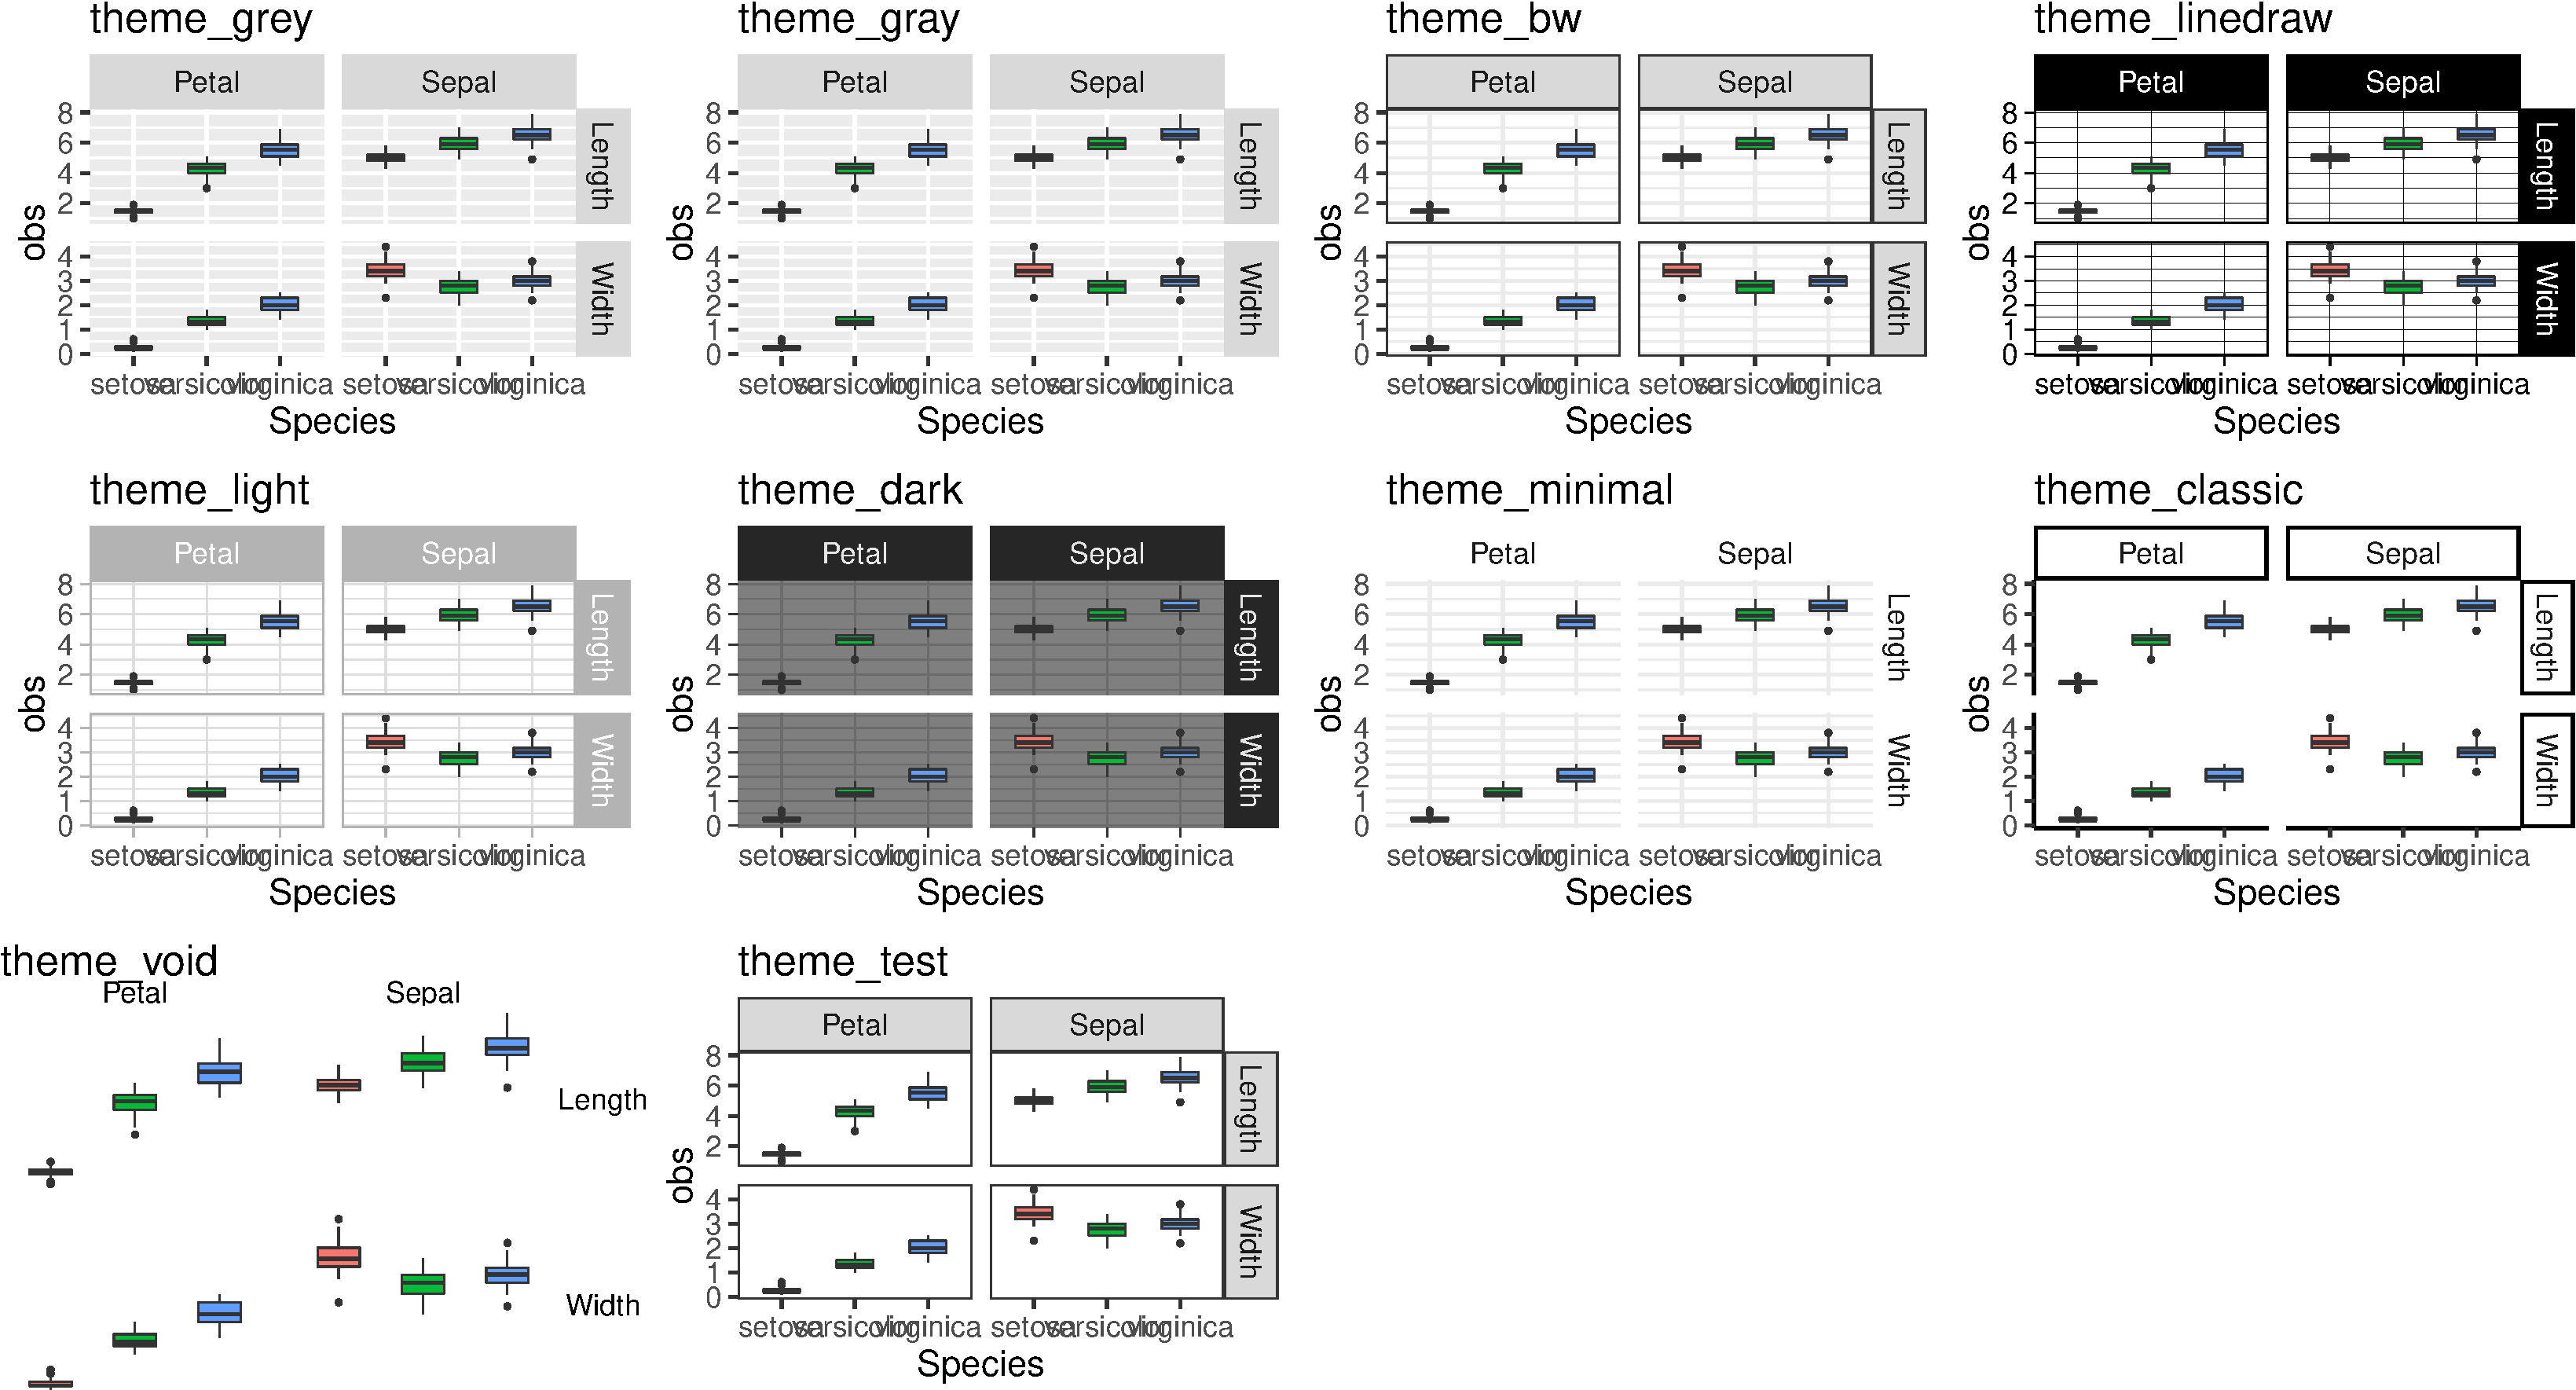
\includegraphics{tidyverse_28_03_files/figure-beamer/ggplot16-1.pdf}

\end{frame}

\begin{frame}{Themes}

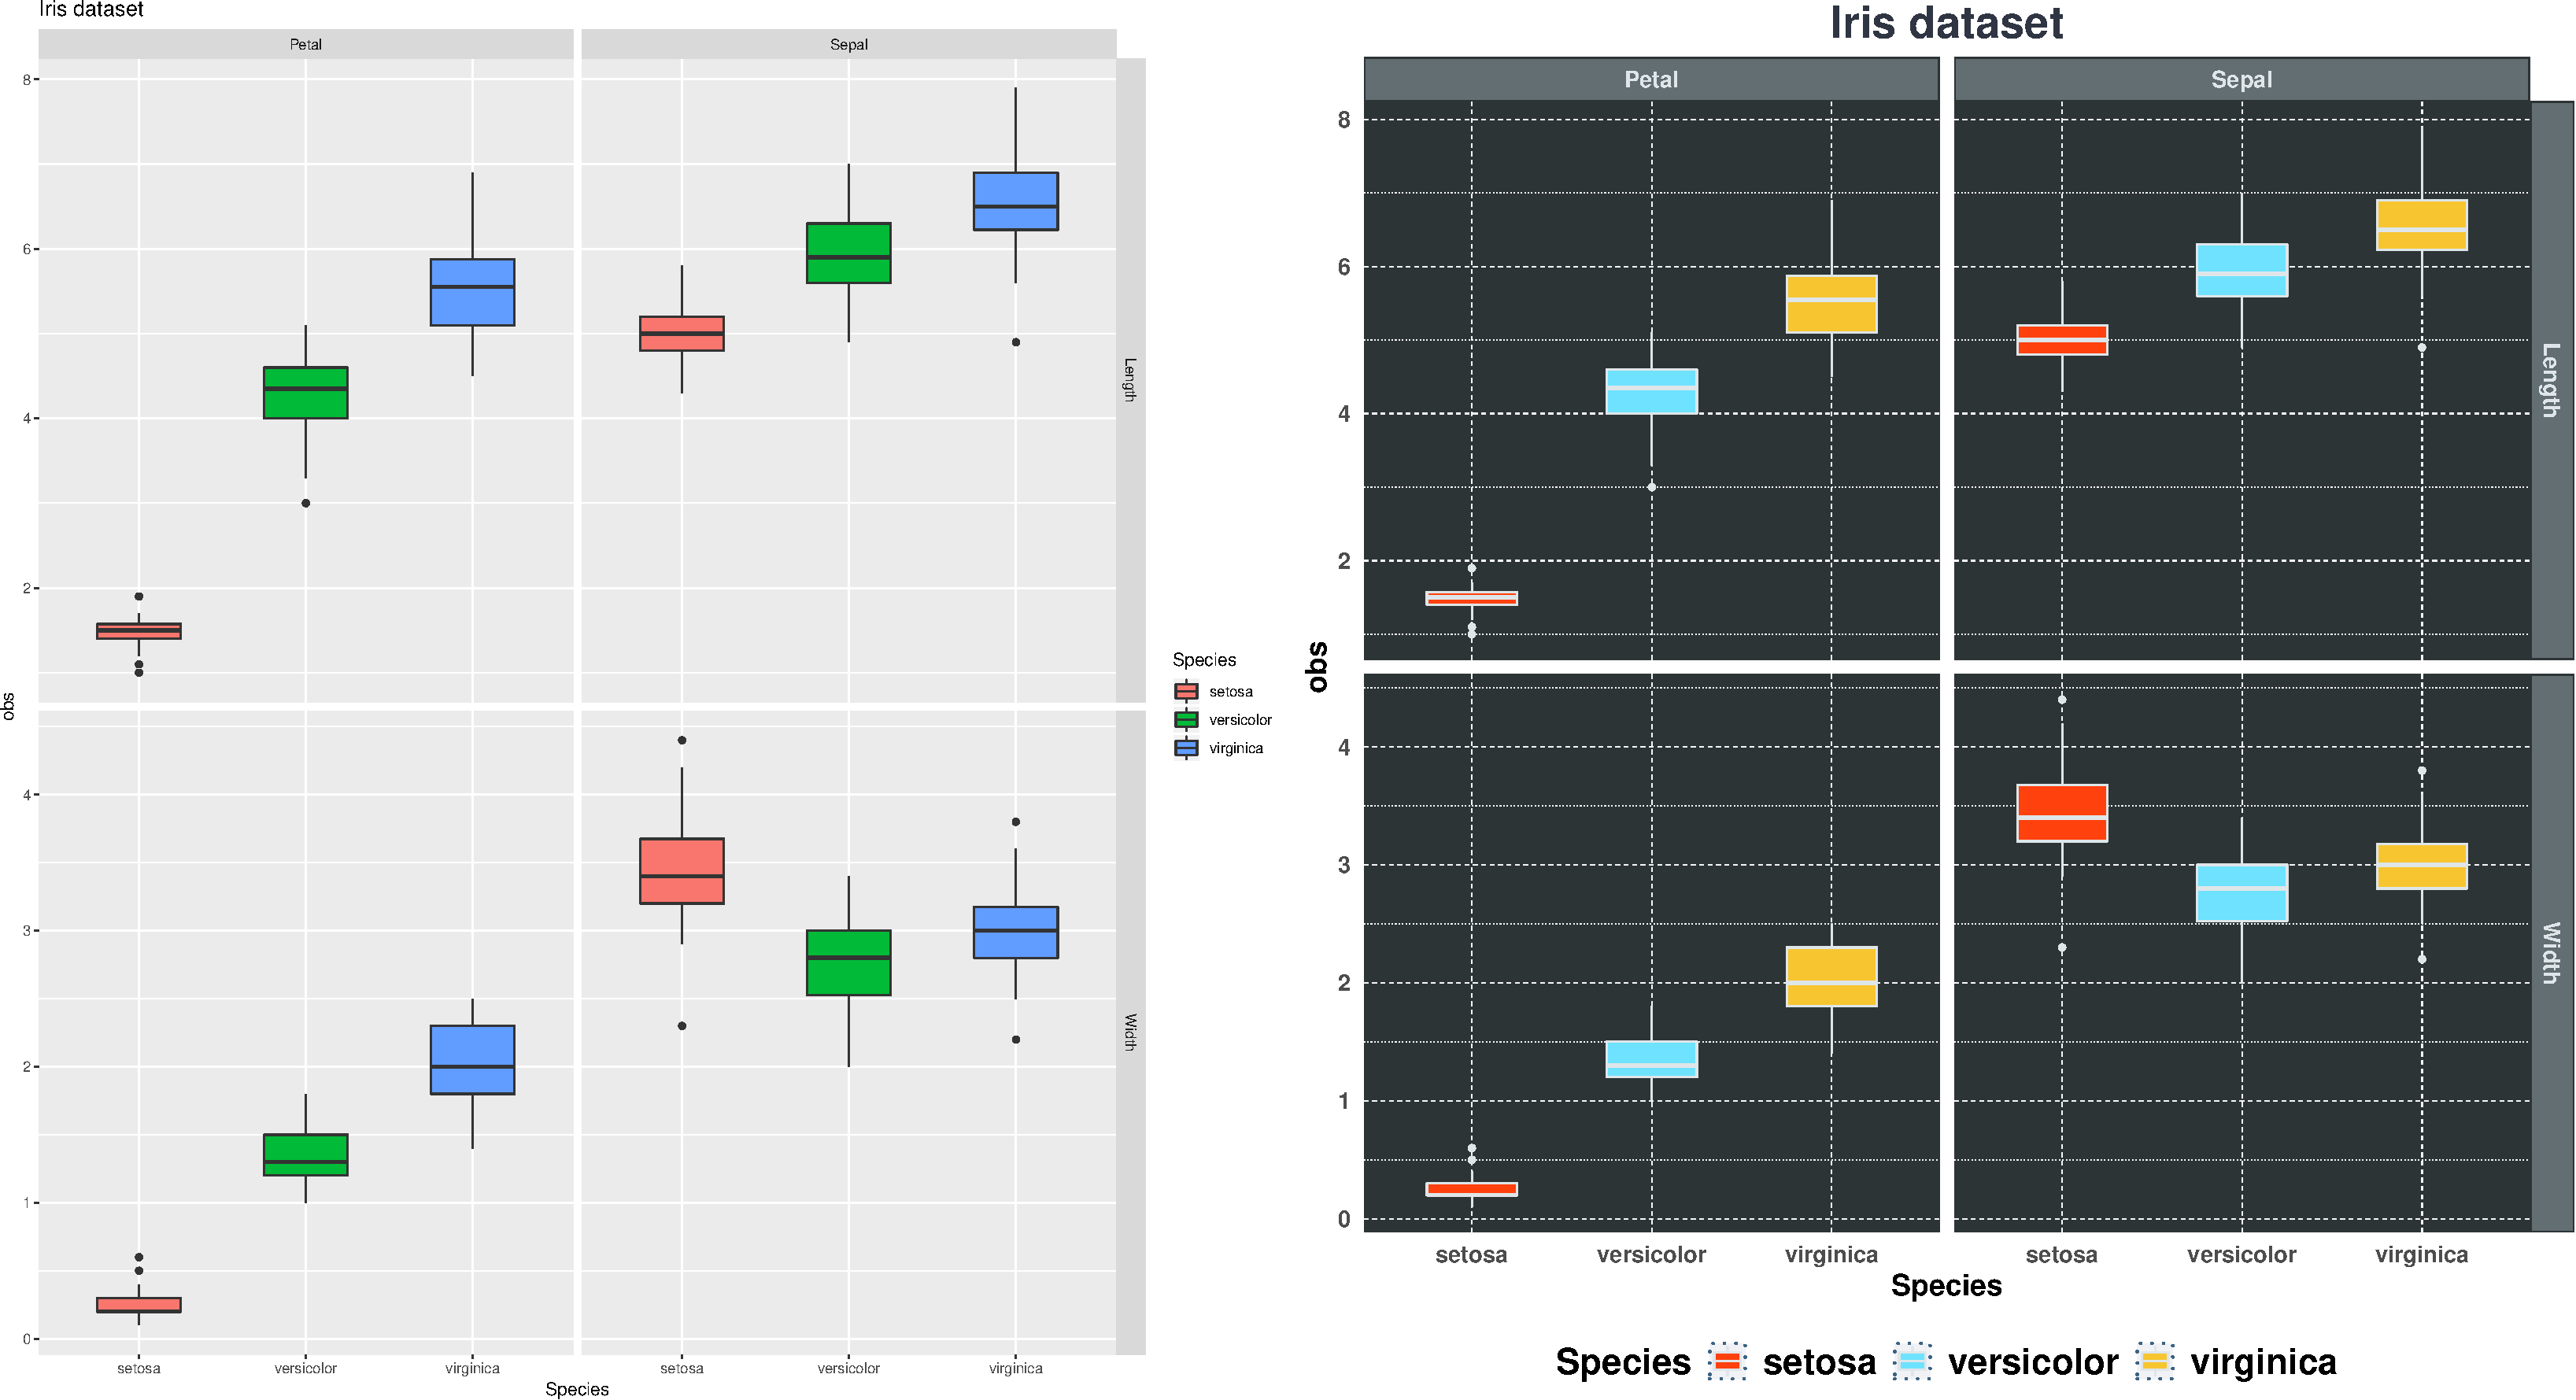
\includegraphics{tidyverse_28_03_files/figure-beamer/ggplot17-1.pdf}

\end{frame}

\begin{frame}{Extensions}

\Large

\begin{itemize}
\tightlist
\item
  \textbf{ggplot2} extensions: This site tracks and lists ggplot2
  extensions developed by R users in the community.
  \url{https://www.ggplot2-exts.org/}.
\item
  \textbf{cowplot}: Arranging graphs into a grid and improve plot
  design.
\item
  \textbf{ggpubr} \& \_\_ ggstatsplot\_\_: Publication ready plots \&
  add statistical tests.
\item
  \textbf{ggrepel}: Automatic label placement.
\item
  \textbf{esquisse}: Explore and Visualize Your Data Interactively with
  ggplot2.
\item
  \textbf{ggvis}: Create rich interactive graphics with a syntax similar
  in spirit to ggplot2.
\end{itemize}

\end{frame}

\begin{frame}{Why I use \texttt{ggplot2}}

\Large

\begin{itemize}
\tightlist
\item
  The ``default'' output is much nicer than with base graphics.
\item
  Automatic legend, color with mapping to the variables.
\item
  Easy to combine multiple plot.
\item
  Easy facetting.
\item
  A lot of themes.
\item
  A lot of extensions \ldots{}
\end{itemize}

\end{frame}

\begin{frame}{Sources}

\Large

\textbf{Sources:}

\begin{itemize}
\tightlist
\item
  \textbf{PDF and sources:}
  \url{https://github.com/rochevin/tidyverse_journal_club}
\item
  \textbf{Web version:}
  \url{https://rochevin.github.io/tidyverse_journal_club}
\end{itemize}

\end{frame}

\end{document}
